\chapter{Designing a software transaction system}\label{cha:stm}
\epigraphhead[70]{\epigraph{%
Easy things should stay easy, hard things should get easier, and
impossible things should get hard.
}{\textit{Motto for Perl~6 development}}}

In this chapter I detail the design of \apex, a
high-performance software transaction system.  I first present
a methodology for isolating likely transactions from benchmarks.
I then describe the system goals, and use quantitative data from
benchmarks to buttress the design choices.  I formalize an
implementation meeting those goals in the modeling language
Promela.  The correctness of this implementation can be model-checked
using the \Spin tool; the details of this effort are in
\appref{verification}.

After outlining the design of \apex in this chapter, \charef{stmimpl}
discusses its practical implementation.

\section{Finding transactions}\label{sec:auto}
One of the difficulties of proposing a novel language feature is the
lack of benchmarks for its evaluation.  Although there is no existing body of
code that uses transactions, there is a substantial body of
code that uses Java (locking) synchronization.  This thesis
utilizes the \flex compiler \cite{Flex} to
substitute {\tt atomic} blocks (methods) for {\tt
  synchronized} blocks (methods) in order to evaluate the properties
Java transactions are likely to have.  The semantics are not
precisely compatible: the existing \indexed{Java memory model} allows
unsynchronized updates to shared fields to be observed within a
synchronized block, while such updates are never visible to a
transaction expressed with an
{\tt atomic} block.\footnote{The Java 5.0 revision of the Java memory model
\cite{MansonPu01a,MansonPu01b,MansonPuAd05} narrows the semantic gap.
The full memory model includes details---such as \texttt{volatile}
fields---which I do not treat in this work.  \Secref{semantic}
discusses the challenges involved in automatic transactification, and 
\cite{GrossmanMaPu06} contains a fuller discussion of the interactions
between transactions and high-level memory models.}
Despite the differences in semantics, the automatic substitution of
{\tt atomic} for {\tt synchronized} does, in fact, preserve the
correctness of the benchmarks I examine here.

\label{sec:properties}
The initial results of this chapter
explore the implications of exposing the transaction
mechanism to user-level code through a compiler.
I compiled the SPECjvm98 benchmark suite with the \flex Java compiler,
modified to turn synchronized blocks and methods into transactions,
in order to investigate the properties of the transactions in such
``automatically converted'' code.
\Flex performed method cloning to distinguish methods called from
within transactions, and implemented nested locks as a single
transaction around the outermost.\footnote{See
  \secref{synctrans} for more details on this transformation.} I
instrumented this transformed program to produce a trace of
memory references and transaction boundaries for analysis.
I found both large
transactions (involving millions of cache lines) and frequent
transactions (up to 45 million of them).  We will show that these
properties are not unusual for typical applications.

The SPECjvm98 benchmark suite represents a variety of typical Java
applications that use the capabilities of the Java standard library.
Although the SPECjvm98 benchmarks are largely single-threaded, they contain
synchronized code within the thread-safe Java standard libraries which
is transformed into transactions.  Because in
this evaluation I am looking at transaction properties only, the
multithreaded \texttt{227\_mtrt} benchmark is identical to its
serialized version, \texttt{205\_raytrace}.  For consistency, I present
only the latter.

\begin{figure}\sis%
\begin{center}
\begin{tabular}{lrrrr}
        & total      &              & transactional & biggest\\
program & memory ops & transactions & memory ops    & transaction \\\hline
{\tt 201\_compress} & 2,981,777,890 & 2,272 & $<$0.1\% & 2,302 \\
{\tt 202\_jess} & 405,153,255 & 4,892,829 & 9.1\% & 7,092 \\
{\tt 205\_raytrace} & 420,005,763 & 4,177 & 1.7\% & 7,149,099 \\
{\tt 209\_db} & 848,082,597 & 45,222,742 & 23.0\% & 498,349 \\
{\tt 213\_javac} & 472,416,129 & 668 & 99.9\% & 118,041,685 \\
{\tt 222\_mpegaudio} & 2,620,818,169 & 2,991 & $<$0.1\% & 2,281 \\
{\tt 228\_jack} & 187,029,744 & 12,017,041 & 34.2\% & 14,266 \\
\end{tabular}
\end{center}
\caption[Transactification of SPECjvm98 benchmark suite.]%
 {Transactification of SPECjvm98 benchmark suite: resulting
  transaction counts and sizes, compared to total number of memory
  operations (loads and stores).  These numbers represent full input
 size runs.
}\label{fig:perfnums}
\end{figure}
\figput{tr-quad2}{Classification of SPECjvm98 benchmarks into quadrants
based on transaction properties.}

\figref{perfnums} shows the raw sizes and frequency of transactions in
the transactified SPECjvm98 suite.  Because the run times of the
benchmarks are roughly comparable,\footnote{The canonical run times
  used for computation of the Spec ratio range from 380 to 1175
  seconds.  Sorted by run time: \texttt{202\_jess}, 380 s;
  \texttt{213\_javac}, 425 s; \texttt{228\_jack}, 455 s;
  \texttt{227\_mtrt}, 460 s; \texttt{209\_db}, 505 s;
  \texttt{222\_mpegaudio}, 1100 s; \texttt{201\_compress}, 1175 s.}
transaction count is also an indicator of transaction rate.
\figref{tr-quad2} proposes a
taxonomy for Java applications with transactions, grouping the SPECjvm98
applications into quadrants based on the number and size of the
transactions that they perform.  Applications in Quads II and IV
require an efficient transaction implementation, because they contain
many transactional operations.
Quads III and IV contain at least some large transactions, which
pose difficulties for currently proposed hardware transactional memory
schemes.  We now
examine the benchmarks in each quadrant to determine why its program
logic caused it to be classified in that quadrant.

Quad I applications perform few (up to about 2000) small
transactions.  These applications include \texttt{201\_compress}, an
implementation of gzip compression, and \texttt{222\_mpegaudio}, an
MP3 decoder.  Both of these applications perform inherently serial
tasks.  They perform quite well with locks, and would likely execute
with acceptable performance even with a \naive software
implementation of transactions, as long as the impact on
nontransactional operations was minimal.

Quad II applications perform a large number of small transactions.
The expert system \texttt{202\_jess} falls in this category, as does
the parser generator \texttt{228\_jack} and
small input sizes of \texttt{209\_db}, a database.  These benchmarks
perform at least an order of magnitude more transactions than Quad
I applications, and all of the transactions are small enough to 
comfortably fit the known hardware transactional memory schemes
\cite[etc]{HerlihyMo93}, if
one were to be implemented.

Quad III includes \texttt{205\_raytrace}, a ray-tracing renderer.  A
small number of transactions are performed, but they may grow
large.  Existing bounded hardware transactional schemes do not
suffice.  The large
transactions may account for a large percentage of total memory
operations, which may make software schemes
impractical.

Finally, Quad IV applications such as \texttt{209\_db} and the
\texttt{213\_javac} Java compiler application perform a large number
of transactional memory operations with at least a few large transactions.  

The \texttt{213\_javac} Java compiler application and the large input
size of the \texttt{209\_db} benchmark illustrate that some programs
contain \emph{extremely} large transactions.  When \texttt{213\_javac}
is run on its full input set, it contains 4 huge transactions,
each of which contains over 118 million transactional memory
operations.  Closer
examination reveals that the method \texttt{Javac.compile()}, which
implements the entire compilation process, is marked as synchronized:
the programmer has explicitly requested that the entire compilation
occur atomically.

The large transactions in Quad III and IV may be, as in this case, a result of
overly coarse-grained locking, but my goal is to
relieve the programmer from the burden of specifying correct
atomic regions of smaller granularity.  Performance may benefit from
narrowing the atomic regions, but execution with coarse regions should
be possible and not prohibitively slow.

The \texttt{209\_db} benchmark suffers from a different problem: at one
point the benchmark atomically scans an index vector and removes an
element, creating a potentially large transaction if the index is
large.  The size of this index is correlated in these benchmarks with
the input size, but it need not be: a large input could still result
in a small index, and (to some degree) vice-versa.

A similar situation arises in the {\tt java.lang.StringBuffer} code
shown in \secref{stringbuffer}:  a call to the synchronized
\texttt{sb.getChars()} method means that
the size of the transaction for this method grows like the length
of the parameter~\texttt{sb}.  In other words, the transaction can be
made arbitrarily large by increasing the length of \texttt{sb}; or,
equivalently, there is no bound on transaction size without a bound on
the size of the string~\texttt{sb}.

\epsfigput[Distribution of transaction size in the SPECjvm98 benchmark
  suite.]{tr-sz-all-1}{Distribution of transaction size in the
  SPECjvm98 benchmark suite.  The x-axis uses a logarithmic
  scale.}

Any transaction system that allows the programmer free reign over specifying
desired transaction and/or atomicity properties will result
in some applications in each of these categories.  Large transactions,
for example, are a side-effect of modularity: when a cross-module call
occurs inside a transaction, the abstraction boundary prevents precise
knowledge of the memory accesses implicitly included.  Existing
hardware transactional memory schemes only efficiently handle
relatively short-lived and small transactions (Quad I or II),
although they are efficient for these transactions.  Object-based
transaction systems can asymptotically approach that efficiency for
long-lived transactions;  the existence of which is shown in
\figref{tr-sz-all-1}, which plots
the distribution of transaction sizes in SPECjvm98
on a semi-log scale.


\vspace*{5mm}

These initial results indicate that real applications can be
transactified with modest effort, yielding significant gains in
concurrency.  In other work \cite{AnanianAsKuLeLi05} we have shown
that a factor of 4 increase in concurrency can be obtained
by doing nothing more than converting locks to transactions.  Since
the transactified applications may contain large transactions, prior
proposed hardware support for transactions is inadequate.


\section{Designing efficient transactions}\label{sec:efficient}

In this section I briefly describe the desired properties of the
\apex software transaction system: strong atomicity,
object-orientation, low bloat, and fast reads.  Where possible I
justify these desiderata using quantitative data obtained from
analyses of the SpecJVM98 benchmarks, which I implemented using the
\flex Java compiler framework.

\subsection{Weak vs.\ strong atomicity}
As previously discussed in \secref{strongatom},
\defn{strongly atomic}\index{Strong atomicity}\index{Atomicity!strong}
transaction systems protect transactions from interference from
nontransactional code, while \defn{weakly atomic} transaction
systems do not afford this protection.
\index{Weak atomicity}\index{Atomicity!weak}
Consider unsynchronized code directly altering the length field of
the {\tt String\-Buffer} class, the example discussed in \secref{stringbuffer}.
In a weakly atomic system, an unsynchronized decrement to the \texttt{count}
field between labels A and B in \texttt{StringBuffer.append()} on
page \pageref{pg:stringbuffer} causes a
\texttt{String\-Index\-Out\-Of\-Bound\-Exception} to be thrown in the call to
\texttt{getChars()} at label B\@.  This exception should never be thrown
by an atomic execution of {\tt String\-Buffer.append()}.

Current software transaction systems implement
only weak atomicity because of the assumed expense of implementing
strong atomicity.  The \apex system
achieves strong atomicity without adding excessive overhead, so that
correct operation is assured even despite concurrent nontransactional
operations on locations involved in a transaction.

\subsection{Object-oriented vs. flat TM}
The \apex transaction system, unlike most current proposals
\cite{HarrisFr03,HerlihyMo93}\note{Include more} (including the
UTM and LTM hardware systems presented in \charef{htm}), uses an
``object-oriented'' design.  Much contemporary research is focused on
implementing a flat (transactional) memory abstraction in software,
primarily because flat systems side-step the large object issues
presented in \charef{largeobj}.  The object-oriented approach, however, offers
several benefits:
\begin{description}
\item[Efficient execution of long-running transactions.]  As discussed
  briefly in Sections \ref{sec:efficiency} and \ref{sec:tm}, flat
  word-oriented transaction schemes typically require overhead proportional to
  the number of words read/written in the transaction, even if these
  locations have been accessed before inside the transaction. Object-oriented
  schemes impose a cost proportional to the number of \emph{objects}
  touched by the transaction---but once the cost of ``opening'' those
  objects is paid, the transaction can continue to work indefinitely
  upon those objects without paying any further penalty.
  Object-oriented schemes are thus seen to be more efficient for
  \emph{long-running transactions}.
\item[Preservation of optimization opportunities.]  Furthermore,
  transaction-local objects can be identified (statically or
  dynamically) and creation/updates to these objects can be done
  without any transaction tax at all.  Word oriented schemes discard
  the high-level information required to implement these optimizations.
%\item[Freedom from implementation restrictions.]
% thinking of multi-version consistency here.
\end{description}
I contend that the problems with previous object-oriented schemes can
be solved while preserving the inherent benefits of an object-oriented
approach, and the current thesis presents one such solution.

\epsbigfigput{bloat-color}{Application slowdown with increasing object bloat
for the SPECjvm98 benchmark applications.}
\subsection{Tolerable limits for object expansion}
An object-oriented transaction scheme requires transaction state
information about each object.  In \apex, this information is added
directly to the objects, to eliminate indirection cost.
I measured the slowdown caused by various
amounts of object ``bloat'' to determine reasonable bounds on the
size of this extra information.  \figref{bloat-color} presents these
results for the SPECjvm98 applications; I determined that two words
(eight bytes) of additional storage per object would not impact
performance unreasonably.  This amount of bloat causes a geometric
mean of 2\% slowdown on these benchmarks.

\begin{figure}\sis%
\begin{center}
\begin{tabular}{lrrrr}
        & transactional & transactional\\
program & memory ops    & stores \% \\\hline
{\tt 201\_compress} & 50,029 & 26.2\% \\
{\tt 202\_jess} & 36,701,037 & 0.6\% \\
{\tt 205\_raytrace} & 7,294,648 & 23.2\% \\
{\tt 209\_db} & 195,374,420 & 6.3\% \\
{\tt 213\_javac} & 472,134,289 & 22.9\% \\
{\tt 222\_mpegaudio} & 41,422 & 18.6\% \\
{\tt 228\_jack} & 63,912,386 & 17.0\% \\
\end{tabular}
\end{center}
\caption{Comparison of loads and stores inside transactions for the
  SPECjvm98 benchmark suite, full input runs.}
\label{fig:writepercent}
\end{figure}
\subsection{Designing for reads vs. writes}
I also measured the number and types of reads and writes for the
SpecJVM98 benchmarks.
\figref{writepercent} shows that transactional reads typically
outnumber transactional writes by at least 4 to 1; in some cases reads
outnumber writes by over 100 to 1.\footnote{The typical ratio roughly
  matches the 3:1 average observed in Hennessy and Patterson
  \cite[pp. 105, 379]{HennessyPa96}.}  It is worthwhile, therefore, to
make reads more efficient than writes.  In particular, since the
flag-overwrite technique discussed in \secref{flagfield} requires us
to allocate additional memory to store the ``real'' value of the
field, I wish to avoid this process for transactional reads,
reserving the extra allocation effort for transactional writes.

\subsection{The big idea: waving FLAGs}\label{sec:flagfield}

\note{Missing: performance numbers for adding check.  Use ``no trans''
version of transaction app and add check into the access functions.}
\note{No: use microbenchmark from later section.}
I would like nontransactional code to execute with minimal overhead,
but transactions should still appear atomic to nontransactional
code.  My basic mechanism is loosely based on the
distributed shared memory implementation of Scales and Gharachorloo
\cite{ScalesGh97}.  I pick a special ``flag'' value, and
``cross-out'' locations currently involved in a transaction by
overwriting them with the flag value.  Reading or attempting to
overwrite a flagged value indicates to nontransactional code
that exceptional processing is necessary; all other nontransactional
operations proceed as usual.  The flagged field either is currently
involved in an active transaction, belongs to a committed or aborted
transaction and requires copy back, or indicates a ``false flag'', a
field with a true value equal to the flag value (see
page \pageref{pg:falseflag}).

This technique explicitly allows safe access to fields
involved in a transaction from nontransactional code, which provides
strong atomicity, a
design goal of the system.
\punt{Strong atomicity eases ``transactification''
of legacy code (but see \secref{semantic}!).}

\section{Specifying the basic mechanism}
I now present algorithms that have these desired properties.
The \apex algorithms provide strongly-atomic object-oriented
transactions with low bloat and fast reads.  Further, the \apex
algorithms are completely nonblocking, which allows good
scaling and proper fault-tolerant behavior.  Specifically, one faulty or slow
processor cannot hold up the remaining good processors.

I implement the synchronization required by the \apex algorithms using
load-linked/store-conditional instructions.  I require a particular
variant of these instructions that allows the location of the
load-linked to be different from the target of the store-conditional.
This variant is supported on many chips in the PowerPC processor family,
although it has been deprecated in version 2.02 of the PowerPC
architecture standard.\footnote{Version 2.02 of the PowerPC
architecture standard says, ``If a reservation exists but the storage
location specified by the \texttt{stwcx.}\ is not the same as the
location specified by the \textit{Load And Reserve} instruction that
established the reservation\ldots it is undefined whether [the operand
is] stored into the word in storage addressed by [the specified
effective address]'' and states that the condition code indicating a
successful store is also undefined in this circumstance \cite[p 25]{PPCII202}.
The user manual for the MPC7447/7457 (``G4'') PowerPC chips states,
however, ``The \texttt{stwcx.}\ instruction does not check the
reservation for a matching address.  The \texttt{stwcx.}\ instruction
is only required to determine whether a reservation exists.  The
\texttt{stwcx.}\ instruction performs a store word operation only if
the reservation exists,'' \cite[Section 3.3.3.6]{MPC7450UM} which is
the behavior we require.  I believe version 1.10 of the PowerPC
Architecture specification required this behavior, although I have not
been able to locate a copy to confirm this requirement.  The Cell architecture specification
follows version 2.02 of the PowerPC specification, although it adds
cache-line reservation operations that can also be used to
implement our algorithm for reasonably-sized objects aligned within
cache lines; see \cite{WitchelLaAnAs01} for an implementation of Java
I created that observes the appropriate alignments.}  This disjoint location
capability is essential to allow us to keep a finger on one location
while modifying another: a poor man's ``Double Compare And Swap''
instruction.

I describe the \apex algorithms in the Promela modeling language
\cite{Holzmann03},
which I used to allow mechanical model checking of the race-safety
and correctness of the design.  Portions of the model have been
abbreviated for this presentation;  the full Promela model is
given in \appref{verification}, along with a brief primer on Promela
syntax and semantics.

%\subsecput{interface}{Interface}
\subsection{Object structures}%datastruct
\figput[Implementing software transactions with version lists.]{tr-multi-obj-big}%
 {Implementing software transactions with version
  lists.  A transaction object consists of a single field {\it
    status}, which indicates if it has COMMITTED, ABORTED, or is WAITING\@.
  Each object contains two extra fields: {\it readers}, a
  singly-linked list of transactions that have read this object; and
  {\it versions} a linked list of version objects.  If an object field
  is \FLAG, then the value for the field is obtained from the
  appropriate linked version object.}
\figref{tr-multi-obj-big} illustrates the basic data structures of the \apex
software transaction implementation.  Objects are extended with two
additional fields.  The first field, {\tt versions}, points to a
singly linked list of object versions.  Each one contains field values
corresponding to a committed, aborted, or in-progress transaction,
identified by its {\tt owner} field.  There is a single unique
transaction object for each transaction.

The other added field, {\tt readers}, points to a singly linked list
of transactions that have read from this object.  Committed and
aborted transactions are pruned from this list.  The {\tt readers}
field is used to ensure that a transaction does not operate with
out-of-date values if the object is later written
nontransactionally.

There is a special flag value, here denoted by \FLAG\@.  It should be
an uncommon value, i.e. not a small positive or negative integer
constant, nor zero.  In my implementation, I have chosen the byte
\texttt{0xCA} to be the flag value, repeated as necessary to fill out
the width of the appropriate type.
The semantic value of an object field is the value in the original
object structure, \emph{unless that value is \FLAG}, in which
case the field's value is the value of the field in the first
committed transaction in the object's version list.  A ``false flag''
occurs when the application wishes to ``really'' store the value \FLAG
in a field. To do so we create a fully-committed version
attached to the object and store \FLAG in that version, as well as in
the object field.\label{pg:falseflag}

\begin{figure}
\sis\fontsize{9}{10}
\begin{verbatim}
#define FLAG 202 /* special value to represent 'not here' */

typedef Object {
  byte version;
  byte readerList; /* we do LL and CAS operations on this field */
  pid fieldLock[NUM_FIELDS]; /* we do LL operations on fields */
  byte field[NUM_FIELDS];
};
typedef Versi0n { /* 'Version' misspelled because SPIN #define's it. */
  byte owner;
  byte next;
  byte field[NUM_FIELDS];
};
typedef ReaderList {
  byte transid;
  byte next;
};
mtype = { waiting, committed, aborted };
typedef TransID {
  mtype status;
};
\end{verbatim}
\caption[Declaring objects with version lists in Promela.]
 {Declaring objects with version lists in Promela.
  The \texttt{byte} datatype encodes pointers.
  The \texttt{fieldLock} field assists in the implementation of the
  load-linked/store-conditional pair of operations in Promela.}
\label{fig:promdecl}
\end{figure}

\figref{promdecl} declares these object structures in Promela.

\subsection{Operations}%ops
I support transactional read/write and nontransactional read/write
as well as transaction begin, transaction abort, and transaction
commit.  Transaction begin simply involves the creation of a new
transaction identifier object.  Transaction commit and abort are simply
compare-and-swap operations that atomically set the transaction object's {\tt
  status} field appropriately if and only if it was previously in the
WAITING state.
The simplicity of commit and abort are appealing: the \apex algorithm
requires no complicated processing, delay, roll-back or validate
procedure to commit or abort a transaction.

I could support nontransactional read and write (that is,
reads and writes that take place outside of any transaction) by
creating a new short transaction that encloses only the single
read or write.  Since nontransactional accesses to objects can be
frequent, I provide more efficient implementations with
the same semantics.

I now present the operations one-by-one.

\subsubsection{Nontransactional read}

The {\tt readNT} function performs a nontransactional read of field $f$ from
object $o$, putting the result in $v$.  
In the common case, the only overhead is to check that
the read value is not \FLAG\@.  If the value read \emph{is}
\FLAG, however, we copy back the field value 
from the most-recently committed transaction (aborting all other
transactions) and try again.  The copy-back procedure notifies
the caller if this is a ``false flag'', in which case the value of this
field really is \FLAG\@.  We pass the {\tt kill\_writers} constant
to the copy-back procedure to
indicate that only transactional writers need be aborted, not
transactional readers.
All possible races are confined to the copy-back procedure, which I
describe on page \pageref{sec:copyback}.

\begin{figure}
\begin{inlinecode}
inline readNT(o, f, v) {
  do
  :: v = object[o].field[f];
     if
     :: (v!=FLAG) -> break /* done! */
     :: else
     fi;
     copyBackField(o, f, kill_writers, _st);
     if
     :: (_st==false_flag) ->
        v = FLAG;
        break
     :: else
     fi
  od
}

inline writeNT(o, f, nval) {
  if
  :: (nval != FLAG) ->
     do
     :: atomic {
          if /* this is a LL(readerList)/SC(field) */
          :: (object[o].readerList == NIL) ->
             object[o].fieldLock[f] = _thread_id;
             object[o].field[f] = nval;
             break /* success! */
          :: else
          fi
        }
        /* unsuccessful SC */
        copyBackField(o, f, kill_all, _st)
     od
  :: else -> /* create false flag */
     /* implement this as a short *transactional* write. */
     /* start a new transaction, write FLAG, commit the */
     /* transaction; repeat until successful. */
     /* Implementation elided. */
     ...
  fi;
}
\end{inlinecode}
\caption{Promela specification of nontransactional read and write operations.}
\label{fig:promrwnt}
\end{figure}
The top of \figref{promrwnt} specifies the nontransactional read operation in
Promela.

\subsubsection{Nontransactional write}
The {\tt writeNT} function performs a nontransactional write of new value $nval$
to field $f$ of object $o$.  For correctness, we must ensure that
the reader list is empty before we do the write.  I implement this check
with a load-linked/store-conditional pair, which is modeled in
Promela slightly differently, ensuring that the write only succeeds
so long as the reader list remains empty.\footnote{A
  standard CAS would not suffice, as the load-linked targets a
  different location than the store-conditional.}
If it is not empty, we
call the copy-back procedure (as in {\tt readNT}), passing the
constant {\tt kill\_all} to indicate that both transactional readers
and writers should be aborted during the copy-back.  The copy-back
procedure leaves the reader list empty.

If the value to be written is actually the \FLAG value, things get a
little bit trickier.  This case does not occur often, and so the
simplest correct implementation is to treat this nontransactional
write as a short transactional write, creating a new transaction for
this one write, and attempting to commit it immediately after the
write.  This implementation is slow, but adequate for this uncommon case.

The bottom of \figref{promrwnt} specifies the nontransactional
write operation in Promela.

\subsubsection{Field Copy-Back}\label{sec:copyback}
\begin{figure}\sis\fontsize{9}{10}
\begin{verbatim}
inline copyBackField(o, f, mode, st) {
  _nonceV=NIL; _ver = NIL; _r = NIL; st = success;
  /* try to abort each version.  when abort fails, we've got a committed
   * version. */
  do
  :: _ver = object[o].version;
     if
     :: (_ver==NIL) ->
        st = saw_race; break /* someone's done the copyback for us */
     :: else
     fi;
      /* move owner to local var to avoid races
       * (owner set to NIL behind our back) */
     _tmp_tid=version[_ver].owner;
     tryToAbort(_tmp_tid);
     if
     :: (_tmp_tid==NIL || transid[_tmp_tid].status==committed) ->
        break /* found a committed version */
     :: else
     fi;
     /* link out an aborted version */
     assert(transid[_tmp_tid].status==aborted);
     CAS_Version(object[o].version, _ver, version[_ver].next, _);
  od;
  /* okay, link in our nonce.  this will prevent others from doing the
   * copyback. */
  if
  :: (st==success) ->
     assert (_ver!=NIL);
     allocVersion(_retval, _nonceV, aborted_tid, _ver);
     CAS_Version(object[o].version, _ver, _nonceV, _cas_stat);
     if
     :: (!_cas_stat) ->
        st = saw_race_cleanup
     :: else
     fi
  :: else
  fi;
  /* check that no one's beaten us to the copy back, then kill readers. */
  checkCopyAndKill(o,f,mode,st);
  /* done */
}
\end{verbatim}
\caption[First half of the field copy-back routine.]
{First half of the field copy-back routine.  The final steps
  have been split off into \texttt{checkCopyAndKill}, which is
  presented in \figref{copyback2}.}\label{fig:copyback1}
\end{figure}
\begin{figure}\sis\fontsize{9}{10}
\begin{verbatim}
inline checkCopyAndKill(o, f, mode, st) {
  /* check that no one's beaten us to the copy back */
  if
  :: (st==success) ->
     if
     :: (object[o].field[f]==FLAG) ->
        _val = version[_ver].field[f];
        if
        :: (_val==FLAG) -> /* false flag... */
           st = false_flag /* ...no copy back needed */
        :: else -> /* not a false flag */
           d_step { /* LL/SC */
             if
             :: (object[o].version == _nonceV) ->
                object[o].fieldLock[f] = _thread_id;
                object[o].field[f] = _val;
             :: else /* hmm, fail.  Must retry. */
                st = saw_race_cleanup /* need to clean up nonce */
             fi
           }
        fi
     :: else /* may arrive here because of readT, which doesn't set _val=FLAG*/
        st = saw_race_cleanup /* need to clean up nonce */
     fi
  :: else /* !success */
  fi;
  /* always kill readers, whether successful or not.  This ensures that we
   * make progress if called from writeNT after a readNT sets readerList
   * non-null without changing FLAG to _val (see immediately above; st will
   * equal saw_race_cleanup in this scenario). */
  if
  :: (mode == kill_all) ->
     killAllReaders(o, _r); /* see Appendix for details */
  :: else /* no more killing needed. */
  fi;
  /* done */
}
\end{verbatim}
\caption[Final portion of the field copy-back routine.]
 {Final portion of the field copy-back routine of \figref{copyback1}.}
\label{fig:copyback2}
\end{figure}
Figures \ref{fig:copyback1} and \ref{fig:copyback2} present the field copy-back routine.  We create a
new version owned by a pre-aborted transaction which serves as a
reservation on the head of the version list.  We then write to the
object field with a load-linked/store-conditional pair if and only if
our version is still at the head of the versions list.\footnote{Again,
  a CAS does not suffice.}  This addresses
the major race possible in this routine.

\subsubsection{Transactional Read}\label{sec:readT}
A transactional read is split into two parts.  The first part, which
occurs before the read, is encapsulated in a routine named
\texttt{ensureReader}.  Its primary task is to
ensure that our transaction is on the reader list for the
object.  This check is straightforward to do in a nonblocking manner as
long as we always add readers to the head of the list.  The
\texttt{ensureReader} routine must also
walk the versions list to abort any uncommitted transaction other
than our own.  Since the \texttt{ensureReader} depends only on the
object involved, not the precise field, redundant read checks for
different fields in the object can be combined and hoisted so that 
\texttt{ensureReader} is performed
once before the first read from an object and not repeated.

At read time, we initially read from the original object.  If the
value read is not \FLAG, we use it.  Otherwise, we look up the version
object associated with our transaction (our version is typically at the
head of the version list) and read the appropriate value from that
version.  The initial read-and-check can be omitted if we
know that we have already written to this field inside this transaction.

\begin{figure}
\begin{inlinecode}
inline readT(tid, o, f, ver, result) {
  do
  ::
     /* we should always either be on the readerList or
      * aborted here */
     result = object[o].field[f];
     if
     :: (result==FLAG) ->
        if
        :: (ver!=NIL) ->
           result = version[ver].field[f];
           break /* done! */
        :: else ->
           findVersion(tid, o, ver);
           if
           :: (ver==NIL) ->/*use val from committed vers.*/
              assert (_r!=NIL);
              result = version[_r].field[f];/*false flag?*/
              moveVersion(_r, NIL);
              break /* done */
           :: else /* try, try, again */
           fi
        fi
     :: else -> break /* done! */
     fi
  od
}

inline writeT(ver, f, nval) {
  /* easy enough: */
  version[ver].field[f] = nval;
}
\end{inlinecode}
\caption{Promela specification of transactional read and write operations.}
\label{fig:promrwt}
\end{figure}

The top of \figref{promrwt} specifies read-time portion of the
transactional read operation in
Promela.  The initial \texttt{ensureReader} portion is
straightforward; it is included in \appref{verification}.

\begin{figure}
\sis\fontsize{6.5}{8}
\begin{verbatim}
/* per-object, before write. */
inline ensureWriter(tid, o, ver) {
  assert(tid!=NIL);
  ver = NIL; _r = NIL; _rr = NIL;
  do
  :: assert (ver==NIL);
     findVersion(tid, o, ver);
     if
     :: (ver!=NIL) -> break /* found a writable version for us */
     :: (ver==NIL && _r==NIL) ->
        /* create and link a fully-committed root version, then
         * use this as our base. */
        allocVersion(_retval, _r, NIL, NIL);
        CAS_Version(object[o].version, NIL, _r, _cas_stat)
     :: else ->
        _cas_stat = true
     fi;
     if
     :: (_cas_stat) ->
        /* so far, so good. */
        assert (_r!=NIL);
        assert (version[_r].owner==NIL ||
                transid[version[_r].owner].status==committed);
        /* okay, make new version for this transaction. */
        assert (ver==NIL);
        allocVersion(_retval, ver, tid, _r);
        /* want copy of committed version _r.  No race because
         * we never write to a committed versions. */
        version[ver].field[0] = version[_r].field[0];
        version[ver].field[1] = version[_r].field[1];
        assert(NUM_FIELDS==2); /* else ought to initialize more fields */
        CAS_Version(object[o].version, _r, ver, _cas_stat);
        moveVersion(_r, NIL); /* free _r */
        if
        :: (_cas_stat) ->
           /* kill all readers (except ourself) */
           /* all changes have to be made from the front of the
            * list, so we unlink ourself and then re-add us. */
           do
           :: moveReaderList(_r, object[o].readerList);
              if
              :: (_r==NIL) -> break
              :: (_r!=NIL && readerlist[_r].transid!=tid)->
                 tryToAbort(readerlist[_r].transid)
              :: else
              fi;
              /* link out this reader */
              CAS_Reader(object[o].readerList, _r, readerlist[_r].next, _)
           od;
           /* okay, all pre-existing readers dead & gone. */
           assert(_r==NIL);
           /* link us back in. */
           ensureReaderList(tid, o);
           break
        :: else
        fi;
        /* try again */
     :: else
     fi;
     /* try again from the top */
     moveVersion(ver, NIL)
  od;
  /* done! */
  assert (_r==NIL);
}
\end{verbatim}
\caption{The per-object version-setup routine for transactional writes.}
\label{fig:ensurewriter}
\end{figure}
\begin{figure}
\sis\fontsize{6.5}{8}
\begin{verbatim}
/* per-field, before write. */
inline checkWriteField(o, f) {
  _r = NIL; _rr = NIL;
  do
  ::
     /* set write flag, if not already set */
     _val = object[o].field[f];
     if
     :: (_val==FLAG) ->
        break; /* done! */
     :: else
     fi;
     /* okay, need to set write flag. */
     moveVersion(_rr, object[o].version);
     moveVersion(_r, _rr);
     assert (_r!=NIL);
     do
     :: (_r==NIL) -> break /* done */
     :: else ->
        object[o].fieldLock[f] = _thread_id;
        if
        /* this next check ensures that concurrent copythroughs don't stomp on each other's versions,
         * because the field will become FLAG before any other version will be written. */
        :: (object[o].field[f]==_val) ->
           if
           :: (object[o].version==_rr) ->
              atomic {
                if
                :: (object[o].fieldLock[f]==_thread_id) ->
                   version[_r].field[f] = _val;
                :: else -> break /* abort */
                fi
              }
           :: else -> break /* abort */
           fi
        :: else -> break /* abort */
        fi;
        moveVersion(_r, version[_r].next) /* on to next */
     od;
     if
     :: (_r==NIL) ->
        /* field has been successfully copied to all versions */
        atomic {
          if
          :: (object[o].version==_rr) ->
             assert(object[o].field[f]==_val ||
                    /* we can race with another copythrough and that's okay; the locking strategy
                     * above ensures that we're all writing the same values to all the versions
                     * and not overwriting anything. */
                    object[o].field[f]==FLAG);
             object[o].fieldLock[f]=_thread_id;
             object[o].field[f] = FLAG;
             break; /* success!  done! */
          :: else
          fi
        }
     :: else
     fi
     /* retry */
  od;
  /* clean up */
  moveVersion(_r, NIL);
  moveVersion(_rr, NIL);
}
\end{verbatim}
\caption{The per-field copy-through routine for transactional writes.}
\label{fig:copythrough}
\end{figure}
\subsubsection{Transactional Write}
Again, writes are split in two.  Once for each object, we must traverse
the version list, aborting other versions and locating or creating a
version corresponding to our transaction.  We must also traverse the
reader list, aborting all transactions on the list except ourself.
This portion of the algorithm is shown in the {\tt ensureWriter}
routine in \figref{ensurewriter}.

Once for each field we intend to write, we must perform a
copy-through: copy the object's field value into all the versions and
then write \FLAG to the object's field.  We use
load-linked/store-conditional to update versions only if the object's
field has not already been set to \FLAG behind our backs by another
copy-through.  The {\tt checkWriteField} routine is shown in
\figref{copythrough}.

Then, for each write, we simply write to the identified version, as
shown at the bottom of \figref{promrwt}.

\section{Performance limits for nontransactional code}
\label{sec:counter-bench}
The software transaction system outlined in this section depends on
the insertion of simple read and write checks in nontransactional
code.  The performance of read and write barriers has been
well-studied in the garbage collection community, but our checks are
slightly different: in particular, they are checks on the
\textit{contents} of a memory cell, rather than on its address.  
Thus our checks
introduce a more direct dependency which may affect performance.
Further, our write check involves a LL/SC instruction pair, which may
behave differently from the standard loads and stores used in
barriers.

In this section I use a simple counter microbenchmark to evaluate the
``best worst case'' nontransactional performance of \apex.
It is an idealized ``best case'' in that I don't benchmark
the effects of ``false flags'' or other forays into the transactional
code path, nor do I account for double-word or subword writes,
cache effects due to code duplication, or other details of a real
implementation.  I investigate these effects with full
benchmarks in \secref{full-bench}.  I also freely
optimize down to the assembly level to determine the fundamental
performance limits.  

The tight read/write dependency makes counter increment
a ``worst case'' benchmark, however.  In general,
modern compilers are good at separating reads from writes in
``real'' code to mask load latency, but this particular microbenchmark
cannot be reasonably unrolled to accomplish the separation.  My
conclusions about the fundamental costs of read and write costs should
thus be tempered by the knowledge that some of these costs are in
practice masked by the same standard compiler techniques used to
mitigate memory-access latencies.

\begin{figure}
\sis\fontsize{9}{10}\begin{verbatim}
typedef int32_t field_t;

struct oobj {
  struct version *version;
  struct readerList * volatile readerList;
  volatile field_t field[NUM_FIELDS];
};
void do_bench(struct oobj *obj) {
  int i;
  for (i=0; i<REPETITIONS; i++) {
    field_t v = read(obj, 0);
    v++;
    write(obj, 0, v);
  }
}
\end{verbatim}
\caption{Counter microbenchmark to evaluate read- and write-check
  overhead for nontransactional code.}
\label{fig:counter-bench}
\end{figure}

\begin{figure}
\sis\fontsize{9}{10}\begin{verbatim}
#if !defined(WITH_READ_CHECKS)

static inline field_t read(struct oobj *obj, int idx) {
  field_t val = obj->field[idx];
  return val;
}

#else

static inline field_t read(struct oobj *obj, int idx) {
  field_t val = obj->field[idx];
  if (unlikely(val==FLAG))
    return unusualRead(obj,idx);
  else return val;
}

#endif
\end{verbatim}
\caption{C implementation of read checks for counter microbenchmark.}
\label{fig:counter-read}
\end{figure}

\begin{figure}
\sis\fontsize{9}{10}\begin{verbatim}
#if !defined(WITH_WRITE_CHECKS)

static inline void write(struct oobj *obj, int idx, field_t val) {
  obj->field[idx] = val;
}

#else

static inline void write(struct oobj *obj, int idx, field_t val) {
  if (unlikely(val==FLAG))
    unusualWrite(obj,idx,val); // never called
  else {
    do {
      if (unlikely(NULL != LL(&(obj->readerList)))) {
        unusualWrite(obj,idx,val); // never called
        break;
      }
    } while (unlikely(!SC(&(obj->field[idx]), val)));
  }
}

#endif
\end{verbatim}
\caption{C implementation of write checks for counter microbenchmark.}
\label{fig:counter-write}
\end{figure}

\figref{counter-bench} presents the basic structure of the counter
microbenchmark. The \texttt{read()} and \texttt{write()} methods
have appropriate definitions inlined for each variant of the
benchmark.  The \texttt{readerList} and \texttt{field}
fields of the \texttt{struct oobj} are marked \texttt{volatile} to
prevent the C compiler from optimizing away the accesses we are
interested in benchmarking.  Without these declarations, \texttt{gcc}
4.1.2 optimizes away the entire benchmark loop and replaces it with
a direct addition of \texttt{REPETITIONS}\@.

\figref{counter-read} shows the baseline \texttt{read()}
implementation, which inlines to a single \texttt{lwz} instruction on
PowerPC, along with the C implementation of the read check necessary
for nontransactional code under our transaction system.  We use 
the \texttt{unlikely()} macro, implemented using the
\texttt{gcc} extension \texttt{\_\_builtin\_expect()}, to apply the
appropriate static prediction bits indicating that \texttt{FLAG} is
expected to be an unusual value.  In our microbenchmark, this
prediction is always correct.  The C compiler must still save
whatever registers are necessary to allow the call to
\texttt{unusualRead()}, although this function is never actually called
during the microbenchmark.  The \texttt{unusualRead} function would be
expected to perform the remainder of the \texttt{readNT} algorithm
from \figref{promrwnt}, including looking up and copying back the most
recently-committed value for this field.

\figref{counter-write} shows the equivalent implementation pairs for a
nontransactional write.  The basic implementation inlines to a single
\texttt{stw} instruction.  The write-check version at the bottom must
perform three tests.  First, it must ensure that the value to be
written is not \texttt{FLAG}\@.  If it is, we must use the ``false flag''
mechanism to write it, modeled here by a call to
\texttt{unusualWrite()}.  This check can be optimized away when
writing a constant,\footnote{Hennessy and Patterson indicate that 35\%
  of integer instructions use an immediate operand \cite[p. 78]{HennessyPa96}.
  Their methodology does not
  allow breaking out the percentage of stores specifically.}
 but the \texttt{volatile} declarations ensure that
our benchmark always performs the check.  Second, we must perform
a load-linked of the object's \texttt{readerList} to check that there
are not any current transactional readers of this object.  Last, we
perform a store-conditional of the value we wish to write and check
that it was successful.  Unlike the other two tests, this check
fails occasionally\footnote{Experimentally, about 3,600 times in
  the 1 billion repetitions of the write during the counter microbenchmark.}
 during the benchmark run due to context switches
that may occur between the load-linked and the store-conditional
instructions.

\epsbigfigput[Check overhead for counter microbenchmark]{phd-counter}{%
  Time overhead of read checks, write checks,
  and both read and write checks for nontransactional code, in both a
  pure C implementation and optimized assembly.}

\figref{phd-counter} shows the performance of this benchmark on the
PowerPC hardware fully described in \secref{full-bench}.
Read checks, even in this worst case where the value read is demanded
immediately, only add 14\% overhead.  Write checks are more costly,
due to the load-linked and store-conditional pair.  Specifically, they add 200\%
overhead to the benchmark.  Combining read and write checks yields the
expected 214\% overhead, as our microbenchmark was carefully constructed to
avoid the opportunities for instruction-level parallelism one might
expect in real-world applications.

\begin{figure}
\sis\fontsize{9}{10}\begin{alltt}
\textit{do_bench:              do_bench:
  mflr 0                 mflr 0
  stwu 1,-16(1)          stwu 1,-16(1)
  lis 5,0x3b9a           addi 10,3,8
  li 8,0                 addi 11,3,4
  ori 5,5,51712          stw 0,20(1)
  addi 6,3,4             lis 0,0x3b9a
  addi 7,3,8             ori 0,0,51712
  stw 0,20(1)            mtctr 0
  b .L4                  b .L4
.L22:
  mr 10,6
  mr 11,7              }\textbf{.L5:
.L5:                   0:
  lwarx 0,0,10           lwarx 0,0,11
  cmpwi 7,0,0            cmpwi 0,0
  bne- 7,.L19            beq+ 1f
  stwcx. 9,0,11          b . # stub for unusualWrite branch
  li 0,0               1:stwcx. 9,0,10
  bne- 0f                bne 0b
  li 0,1
0:                       bdz .L14
  cmpwi 7,0,0
  beq- 7,.L5
  addi 8,8,1
  cmpw 7,8,5
  beq- 7,.L21}\textit{
.L4:                   .L4:
  lwz 9,8(3)             lwz 9,8(3)
  cmpwi 7,9,-13623       cmpwi 7,9,-13623
  addi 9,9,1             addi 9,9,1
  bne+ 7,.L22            bne+ 7,.L5
.L21:                  .L14:
  lwz 0,8(3)             lwz 0,8(3)
                         xoris 9,0,0xc465
  cmpw 7,0,8             cmpwi 7,9,-13824
  bne- 7,.L23            bne 7,.L15
  lwz 0,20(1)            lwz 0,20(1)
  addi 1,1,16            addi 1,1,16
  mtlr 0                 mtlr 0             
  blr                    blr}
\end{alltt}
\caption[PowerPC assembly for counter microbenchmark with
  write checks.]{PowerPC assembly for counter microbenchmark with
  write checks.  The right-hand column is generated from the C
  implementation.  The left-hand column has an optimized version of the
  write check inlined into the code using the \texttt{asm} keyword.
  Italicized code is essentially unchanged.  The optimized section is
  shown in boldface.}
\label{fig:write-assem}
\end{figure}
\begin{figure}
\sis\fontsize{9}{10}\begin{verbatim}
    # repetition count is in the count register to start
    b 0f
    .balign 32 # align to 32-byte cache-line boundary
    nop
    nop
    nop
    nop
    nop
    nop
0:  lwarx 5,0,0
    lwz 6, 0(9)
1:  ori 8, 6, 3
    addi 7, 6, 1
    cmpwi 1, 5,0
    cmpwi 2, 8, 0xFFFFCACB
    bne- 1, 0b # stub: unusualWrite
    beq- 2, 0b # stub: unusualRead or unusualWrite
    stwcx. 7,0,9
    lwarx 5,0,0
    lwz 6, 0(9)
    bne- 0, 1b
    bdnz 1b
\end{verbatim}
\caption{Optimized PowerPC assembly for counter microbenchmark with both read
  and write checks.}
\label{fig:rw-assem}
\end{figure}
Examination of the assembly code generated for this simple benchmark
seems to indicate substantial scope for improvement.  The inline
assembly mechanism of \texttt{gcc}/C provides no inherent support for
instructions 
like the PowerPC's ``store-conditional'' (\texttt{stwcx.}) that leave
their results in a condition code register.  \figref{write-assem}
shows the assembly emitted for the write-check version of the
microbenchmark, with the cumbersome mechanism required to move the
condition code to a register so that it can then be retested.  We can
easily hand-code a better write-check mechanism, shown in the
right-hand column of the figure.\footnote{This version has a stub where a
function call to \texttt{unusualWrite} would usually go; the correct
code here would branch to a small thunk that performs the
frame operations and register saves necessary to adhere to the C
calling convention; \texttt{gcc} makes it difficult to ensure that
this thunk is ``near enough'' for a direct branch (within a 24-bit
signed displacement) without duplicating it needlessly.}
The optimized store-conditional test reduces write-check overhead to
186\% and combined read- and write-check overhead to 199\%, as shown
in \figref{phd-counter}.

Further performance improvement is possible by optimizing the
benchmark with both read and write checks as a whole. \figref{rw-assem}
shows an
optimized assembly version of our \texttt{do\_bench()} function.  I've
primarily rescheduled the code here to separate dependent instructions
as much as possible, but I've also ensured repeatable instruction
cache alignment,\footnote{The MPC7447 (G4) PowerPC has a 32-byte cache
  line, although fetches occur in 16-byte (4 instruction) chunks.}
replaced our canonical \texttt{FLAG} value with
\texttt{0xFFFFCACA}, which can be represented by the PowerPC's 16-bit
signed immediate instruction field (eliminating the need for a
register), and combined the flag checks in
the read and write routines.\footnote{Again, the branches to
\texttt{unusualRead()} and 
\texttt{unusualWrite()} are difficult to express in this hybrid of C
and assembly, but small stubs would be written to save registers and
perform a branch with the appropriate calling conventions.}
The read-and-write check overhead is improved to 143\% with these
optimizations.  The remaining overhead is
due mostly to the irreducible dependency between the
load-linked and store-conditional instructions.
\note{It may be worth looking closely at the instruction schedule for
this optimized counter loop to understand the fundamental performance
limits.}

\epsbigfigput[Check overhead as percentage of total dynamic instruction count]
  {phd-counter-instr}{%
  Check overhead as percentage of total dynamic instruction count.
  The bar on the left is the DLX instruction mix for SPECint92 from
  \cite[p.105]{HennessyPa96}.  On the right is the same instruction
  mix after scaling the loads and stores according to
  \figref{phd-counter}.}

Hennessy and Patterson's measurements indicate that load and store
instructions comprise respectively 26\% and 9\% of dynamic instruction
counts in SPECint92 on a RISC microarchitecture (DLX)
\cite[p. 105]{HennessyPa96}.
As a rough estimate, using dynamic instruction count as a proxy for
instruction time,
the 14\% read overhead and 186\% write overhead measured
in this microbenchmark thus translate into 20\% net overhead for
nontransactional code.\footnote{$0.65 + (1.14 \times 0.26) + (2.86
  \times 0.09) = 1.20$} If we conservatively assume that most of the
improvement in \figref{rw-assem}'s optimized checks should be credited
to reduced write-check overhead, giving the same 14\% read overhead
but only 129\% write overhead, the same metric gives only 15\% net
overhead, as shown in \figref{phd-counter-instr}.  This figure should be
considered a rough lower bound for the time overhead, possible with
aggressive optimization and scheduling.\footnote{This
  calculation combines over- and underestimation, making this number
  only a rough bound.  The use of dynamic instruction count, rather
  than dynamic instruction time, likely underestimates the
  contribution of loads and stores to the run time.
  Scheduling, prefetching, and store buffers can pipeline the cost of
  the loads and stores, however, which might cause our overhead estimate to
  exceed the actual cost.  \Secref{full-bench} presents actual
  overhead measurements of real Java applications.}

\section*{Implementation}
Some details are not yet covered by our model.
For example, how are fields of different byte lengths handled?  How does
transactional Java code interact with the garbage collector, or with
native code in the runtime system?  \Charef{stmimpl} addresses the
real-world
implementation details of our software transaction system.

%%%%%%%%%%%%%%%%%%%%%%%%%%%%%%%%%%%%%%%%%%%%%%%%%%%%%%%%%%%%%%%%%%%
\chapter{Implementing efficient software transactions}\label{cha:stmimpl}
\epigraphhead[70]{\epigraph{%
In theory, there is no difference between theory and practice.
}{\textit{Jan~L.~A.~van~de~Snepscheut}}}

This chapter discusses the challenges involved in translating the
design from \charef{stm} to a practical Java
compiler, the implementation techniques I used, and the performance
achieved.  I conclude by listing some limitations of the
implementation, and describing how they may be overcome in a
production-quality compiler.

\section{The \flex compiler infrastructure}
In 1998 I began implementing the \flex compiler infrastructure for
Java \cite{Flex}, which I used to evaluate the transaction system
implementations in this thesis.  \Flex has been used in over 20
published papers
\cite{DallmeierLiWaZe06,AnanianAsKuLeLi06,Ananian05,AnanianAsKuLeLi05,SalcianuRi05,RinardSaBu04,AnanianRi03,BoyapatiSaBeRi03,FeizabadiBeRaLiRi03,GheorghioiuSaRi03,ZeeRi02,WitchelCaAs02,Gheorghioiu02,Francu02,WitchelLaAnAs01,Whaley01,Salcianu01,BeebeeRi01,Beebee01,Klock01,SalcianuRi01,VivienRi01,Ananian99,WhaleyRi99},
on a wide range of topics.

\Flex is a whole-program static compiler for Java with a runtime
system built around the GNU Classpath implementation of the Java
standard libraries \cite{Classpath}.  \Flex takes as input Java
bytecode, generated by any Java 1.0-1.6 compiler from user code and
the GNU Classpath 0.08 library implementation, and it emits either
assembly code for MIPS, Sparc, or StrongARM, or else 
``portable assembly language'' written in \texttt{gcc} 3.4's variant
of C\@.  The emitted code is compiled and linked against the \flex runtime
system and the GNU Classpath 0.08 native libraries to produce a
stand-alone binary for the target system.  The \flex compiler and
analysis code is written in Java, while the \flex runtime system is
written in C\@.

\subsection*{Using C as a target}\label{sec:precisec}
The experiments in this thesis were conducted on either the x86 or
PowerPC architectures, for which \flex does not have a native assembly
backend.  The ``Precise C'' backend was thus used, so named because,
aside from emitting C code, it's original purpose was to investigate
the possibility of precise garbage collection while emitting
high-level code.  To that end, the backend contains code to maintain a
separate stack for values of non-primitive types and to push and pop
all live variables to this stack at gc points.  Since \flex's low-level
IR may create derived pointers that point inside objects, for example
during loop optimizations, the Precise C backend also reconstructs
the derived pointers after the gc point, in case the objects involved
have moved.\label{sec:precise-gc}

Experiments showed that this mechanism has minimal impact on
performance, because variables pushed onto the explicitly managed
``object stack'' are then dead across the call from the perspective
of the underlying C compiler; in effect our explicit stack management
replaced the implicit stack save/restore which the C compiler would
otherwise have performed to maintain its calling convention.

Java exceptions presented another difficulty when implementing a C
backend.  The mechanisms used in our assembly backends (separate
return addresses for ``returning'' an exception, either derived by
rule from the normal return address or stored in a sorted table keyed
by the normal return address) cannot be implemented in C\@.  \Flex supports
two alternate translations: the first uses \texttt{setjmp} and
\texttt{longjmp} to branch directly from the site where the exception
is thrown to an appropriate handler, and the second returns a pair
value from every function call.  In the \texttt{setjmp} method \flex emits
a \texttt{setjmp} call when a new exception-handling region
(\texttt{try}/\texttt{catch} block) is entered and a \texttt{longjmp}
when an exception is thrown,
but \texttt{setjmp} and \texttt{longjmp} are rather
expensive.  The pair-return method returns a C \texttt{struct} from every
call consisting of the ``real'' return value along with an exception
value.\footnote{Methods declared as \texttt{void} return only the
  exception value, of course.}  When the function returns, the caller
must first test the exception value; if it is non-\texttt{NULL}, then
an exception has been thrown and the caller must handle it (if it can)
or re-throw it.
The mandatory test in the pair-return method adds overhead to every
function call, but it is minimal.  

% source of #s in table & next paragraph: mail to Martin in 'harpoon' folder,
% written on Jul 2, 2000; mail from cananian@netwinder2.lcs.mit.edu in
% the 'harpoon' folder, sent on Sep 29, 2000.

\begin{figure}\sis
\begin{center}
\begin{tabular}{lrrr}
          &\multicolumn{3}{c}{execution time (seconds)} \\
benchmark &\multicolumn{1}{c}{assembly}
          &\multicolumn{1}{c}{pair return}
          &\multicolumn{1}{c}{\texttt{setjmp}} \\ \hline
{\tt 201\_compress} &    223.2 &   193.0 &   183.7 \\
{\tt 202\_jess}     &        - &   446.1 &   463.3 \\
{\tt 205\_raytrace} &    265.8 &   854.8 &   858.3 \\
{\tt 209\_db}       &    591.3 &   578.1 &   597.7 \\
{\tt 222\_mpegaudio}&  1,210.3 & 3,035.0 & 3,014.0 \\
{\tt 227\_mtrt}     &    277.0 &   866.0 &   867.9 \\
{\tt 228\_jack}     &    895.7 &   460.1 &   703.0 \\
\end{tabular}
\end{center}
\caption[Speed comparison of exception return techniques for SPECjvm98
  benchmarks.]
{Speed comparison of exception return techniques for SPECjvm98
  benchmarks on a Netwinder platform.
  The Netwinder is a small, low power computing platform
  designed by Corel Computer around the StrongARM 110 processor.
  For the presented results, lower execution time is better.
  The ``assembly'' column uses \flex's StrongARM backend and uses a lookup
  table keyed on the procedure return address to find an appropriate
  exception handler.  The ``pair return'' and ``\texttt{setjmp}''
  columns use \flex's ``Precise C'' backend, and use the
  implementation strategies described in the text.}
\label{fig:setjmp}
\end{figure}

Experiments on x86 indicated that
a small benchmark consisting of 50,000 method calls executed in
2 milliseconds (ms) using pair-return, regardless of whether the calls
returned normally or threw an exception.  The same benchmark
using the \texttt{setjmp} method ran in only 
1ms when all calls returned normally, but took 73ms when
each call threw an exception. As a result,
\texttt{setjmp} is dramatically slower for applications that heavily use
exceptions.  For example, the SPECjvm98 benchmark \texttt{228\_jack}
executes in 460 seconds with pair return, but 703 seconds with
\texttt{setjmp}.  \figref{setjmp} presents full results for the
SPECjvm98 benchmark suite.

The experiments in this thesis all use pair-return to implement
exceptions.  All experiments also use conservative garbage
collection~\cite{BoehmDeWe91}, making the ``Precise C'' stack unnecessary.

\section{Transforming synchronization}\label{sec:synctrans}
Aside from implementing the read and write mechanisms of the software
transaction design presented in the previous chapter, several
other transformations and analyses of our Java benchmarks must be
performed: transactions must be synthesized from the benchmark's
monitor synchronization, methods must be cloned according to the
context (whether inside a transaction or not) of their call site,
and analyses must be performed in order to reduce redundant checks in the
transformed code.  In addition, some minor desugaring is done to ease
implementation.

\subsection{Method transformation}
\begin{figure}\sis\fontsize{9}{10}
\begin{minipage}{1.5in}
\begin{verbatim}
synchronized {
    ...
    x = o.f;
    ...
    o.f = y;
    ...
    z = foo(a, b, c);
    ...
}
\end{verbatim}
\end{minipage}
$\Rightarrow\quad$
\begin{minipage}{3in}
\begin{verbatim}
t = CommitRecord.newTransaction();
while(true) {
  try {
    ...
    v = ensureReader(o, t);
    x = readT(o, FIELD_F, &v, t);
    ...
    v = ensureWriter(o, t);
    checkWriteField(o, FIELD_F);
    writeT(o, FIELD_F, y, v); /* v.f = y */
    ...
    z = foo$$withtrans(t, a, b, c);
    ...
    t.commitTransaction();
    break;
  } catch (TransactionAbortException tex) {
    t = t.retryTransaction();
  }
}
\end{verbatim}
\end{minipage}
\caption[Software transaction transformation.]
{Software transaction transformation.  The code on the left is the
  original Java source; the transformed source is on the right.}
\label{fig:synctrans}\end{figure}

I automatically created transactions in the benchmarks I present from
Java synchronized blocks and methods.  \figref{synctrans} illustrates
the transformation applied.

Entering a top-level synchronized block creates a new transaction
object and starts a new exception handler context.  Exiting the block
causes a call to the transaction's commit method.  If the commit, or
any other operation inside the block, throws
\texttt{TransactionAbortException} indicating that the transaction
must be aborted, we recreate the transaction object and loop to retry
the transaction's operations.  The \texttt{retryTransaction} method
performs backoff.  Although not implemented in this work,
\texttt{retryTransaction} 
may also perform livelock detection or other
transaction management functions.

Inside the transaction context, reads and writes must be transformed.
Before the read, the \texttt{ensureReader} algorithm
must be invoked (see \secref{readT}).  This
is only done once for each object read in this transaction.
\secref{hoist} describes how these checks are hoisted and combined to
reduce their number.  The \texttt{ensureReader} routine returns a
pointer to a \defn{version object} containing this transaction's field
values for the object.  The pointer may be NULL, however, if this
transaction has not written the object.
The actual read is done via the \texttt{readT}
algorithm described in \figref{promrwt} and \secref{readT}; it may
update the cached version object for the given object (for example, if
the object has been written within this transaction since the point at
which \texttt{ensureReader} was invoked).\footnote{Since the \flex
  infrastructure cannot create pointers to temporaries, or
  alternately return multiple values from function calls, the
  version object in my current implementation cannot be updated by
  \texttt{readT}\@.  This limitation impairs the ability to hoist and combine
  \texttt{ensureReader} and requires redundant calls in our current
  implementation.}

Before each write, \texttt{ensureWriter} and \texttt{checkWriteField}
must be executed.  Like \texttt{ensureReader}, \texttt{ensureWriter}
(\figref{ensurewriter}) need only be performed once for each object
written in the transaction, and it is hoisted and combined in the same
way.  \note{Can \texttt{ensureWriter} imply \texttt{ensureReader}?}
The \texttt{checkWriteField} algorithm (\figref{copythrough}) need
only be executed once for each object field written; if the same field
in the same object is written multiple times, the subsequent
\texttt{checkWriteField} invocations can be eliminated.  The actual
write is performed via \texttt{writeT} (\figref{promrwt}), which is a
simple store to the version object.

Nested transactions are implemented via subsumption; that is, nested
synchronized blocks inside a transaction context are ignored: the
inner transaction is subsumed by the outermost.

\label{sec:withtrans}
Method invocations inside transaction context must be transformed,
since read and write operations are implemented differently depending
on whether or not the current execution is inside a transaction.  \Flex
creates a transactional clone from each method, named with a
\texttt{\$\$withtrans} suffix, which is invoked when executing
inside a transaction.  The current transaction is passed as the first
parameter of the cloned method.\footnote{Cloning must take virtual
  dispatch into account: cloning a method in a superclass must also
  create appropriate cloned subclass implementations.}

Nontransactional code inside a method must be transformed to use the
\texttt{readNT} and \texttt{writeNT} mechanisms to perform object
reads and writes (\figref{promrwnt}); the implementation is similar to
that shown in \figref{counter-read} and \figref{counter-write}.

\subsection{Analyses}\label{sec:hoist} % (check/field oracles)
Performance improves if \flex can identify objects or fields
that are guaranteed not to be concurrently mutated and replace the
checks and read/write protocols with direct accesses.  I performed two
analyses of this sort; \secref{moreopt} describes additional analyses
which we have not implemented.

Our first analysis classifies all fields in the program according to
their use in transactional and nontransactional regions.  This
analysis is encapsulated in a \flex class named
\texttt{GlobalFieldOracle}.  Fields that can never be written within
a transaction do not need the special \texttt{readNT} mechanism from
nontransactional code; their values can be loaded directly without
testing for \texttt{FLAG}\@.  The only way that the field can have the
\texttt{FLAG} value, if it is not written within a transaction, is if
it is a false flag, in which case its value really is \texttt{FLAG}\@.
Similarly, fields that can never be read or written within a
transaction do not need to use the \texttt{writeNT} mechanism; they
can just store directly to the field.\footnote{It is not
  enough for the field not to be written; we must also protect against
  write-after-write conflicts.}  Thus, \texttt{GlobalFieldOracle} can
make nontransactional code more efficient by eliminating the overhead
of the software transaction system in some cases.

While \texttt{GlobalFieldOracle} targets nontransactional code, the
\texttt{Check\-Oracle} analysis classes make transactional code more
efficient by removing unneeded read and write checks.  As mentioned
above, the \texttt{ensureReader} and \texttt{ensureWriter} checks need
only be invoked once on each unique object read/written by the
transaction.  Similarly, \texttt{checkWriteField} need only be
performed once on each object field written by the transaction.  The
\texttt{CheckOracle} classes hoist each check to its immediate
dominator~\cite{Offner95,LengauerTa79,Tarjan74}
if and only if this new location for the check is postdominated by the
current location and the new location is dominated by the definition
of the variable referenced in the check.  This condition ensures that all paths
to the original location of the check must pass through the new
location.  Moreover, it ensures that the object involved in the check is still defined
appropriately at the new check location, since the analysis is
performed on a single-assignment intermediate representation
\cite{Ananian99}.  The check-hoisting process is repeated until no
checks can be moved higher, and then \flex eliminates any check that is
dominated by an identical check.

\subsection{Desugaring} % clone/arrayinit
\Flex also desugars some Java idioms to ease implementation.  Java
specifies a \texttt{clone()} method of \texttt{java.lang.Object},
from which every object is derived.  The top-level \texttt{clone()} method is
somewhat magical, as it creates an exact copy of its subclass,
including all its fields, which are otherwise hidden from methods of a
superclass.  The transactional translation of this method is also
somewhat baroque: it would have to mark all fields of the original
method as ``read'' by the transaction, and then construct a versioned
object written by the transaction.  As an end-run around this
complexity, we desugar \texttt{clone()} into individual
implementations in appropriate classes, each of which reads all fields
of the class, and constructs a new object bypassing its
constructors, and then individually sets all the fields to their new
values.  Arrays get a similar \texttt{clone()} implementation that
reads and writes the elements of the array.  These new implementations
can then be transformed by the transaction pass like any other piece
of code that reads and writes fields.

The \flex infrastructure also contains a mechanism for fast
initialization of arrays.  This mechanism is desugared into
individual array set operations so that it, too, can be uniformly
transformed by the transaction pass.

\section{Runtime system implementation}
The \flex runtime system was extended to support transactions.  The
runtime uses the standard Java Native Interface (JNI) \cite{JNI} for
native methods (written in C) called from Java.  Certain parts of the
transaction system were written as native methods invoked via JNI, but
others interact with the runtime system at a much lower level.
  
The runtime system is parameterized to allow a large number of memory
allocation strategies and collectors, but for the experiments reported
here, I used the Boehm-Demers-Weiser conservative garbage collector
\cite{BoehmDeWe91}.\punt{\footnote{The use of a conservative collector means
  that the mechanism described in \secref{precise-gc} to enable
  precise garbage collection was unneeded and thus disabled for these
  experiments.} }
Ideally the garbage collector would know enough about the transaction
implementation to be able to automatically prune unneeded committed or
aborted versions from the object's version list during collection.
\Flex relies on opportunistically nulling out tail pointers
during version list traversal,\footnote{For example, while looking for the
last committed version.} however, which may result in incomplete collections
(and more memory usage than strictly necessary).

Each transaction had a \texttt{CommitRecord} object storing its state,
whether \texttt{COMMITTED}, \texttt{ABORTED}, or still
\texttt{WAITING}\@.  Most \texttt{CommitRecord} methods were written in
Java, including object creation, exponential backoff on retry, and
throwing the appropriate \texttt{TransactionAbortException} on abort.
Only the crucial \texttt{commit()} and \texttt{abort()} operations,
which atomically set the transaction status if and only if it is still
\texttt{WAITING}, were written in C, as JNI methods.

\subsection{Implementing the JNI}
\begin{figure}\sis\fontsize{9}{10}\begin{alltt}
struct JNINativeInterface \{
  \(\cdots\)
  \textit{/* Calling instance methods */}
  jmethodID (*GetMethodID)
    (JNIEnv *env, jclass clazz, const char *name, const char *sig);
  jobject (*CallObjectMethod)
    (JNIEnv *env, jobject obj, jmethodID methodID, ...);
  \(\cdots\)
  jboolean (*CallBooleanMethod)
    (JNIEnv *env, jobject obj, jmethodID methodID, ...);
  \(\cdots\)
  jbyte (*CallByteMethod)
    (JNIEnv *env, jobject obj, jmethodID methodID, ...);
  \(\cdots\)
  \textit{/* Accessing fields of objects */}
  jfieldID (*GetFieldID)
    (JNIEnv *env, jclass clazz, const char *name, const char *sig);
  jobject (*GetObjectField)
    (JNIEnv *env, jobject obj, jfieldID fieldID);
  jboolean (*GetBooleanField)
    (JNIEnv *env, jobject obj, jfieldID fieldID);
  \(\cdots\)
  void (*SetObjectField)
    (JNIEnv *env, jobject obj, jfieldID fieldID, jobject value);
  void (*SetBooleanField)
    (JNIEnv *env, jobject obj, jfieldID fieldID, jboolean value);
  \(\cdots\)
  \textit{/* Array Operations */}
  jobject (*GetObjectArrayElement)
    (JNIEnv *env, jobjectArray array, jsize index);
  void (*SetObjectArrayElement)
    (JNIEnv *env, jobjectArray array, jsize index, jobject value);
  \(\cdots\)
  jboolean* (*GetBooleanArrayElements)
    (JNIEnv *env, jbooleanArray array, jboolean *isCopy);
  jbyte* (*GetByteArrayElements)
    (JNIEnv *env, jbyteArray array, jboolean *isCopy);
  \(\cdots\)
\};
\end{alltt}
\caption[A portion of the Java Native Interface] {A portion of the
  Java Native Interface for interacting with the Java runtime from C
  native methods \cite{JNI}\@.  There are function variants for all of the
  basic Java types: boolean, byte, char, short, int, long, float,
  double, and Object.  The \texttt{jobject} and
  \texttt{j*Array} types are not direct references to the heap
  objects, but rather opaque wrappers that preserve the garbage
  collector's invariants and protect the runtime system's private
  implementation.}
\label{fig:jni}
\end{figure}

No Java transaction implementation is complete without some mechanism
for executing native methods, that is, C code.  One cannot banish all
native methods, since the Java standard library is built on them. 
If one cannot make native code observe the \texttt{readNT} and
\texttt{writeNT} protocols, one must ensure that the native code never
reads any object written in a transaction, or writes any object read
or written in a transaction.\footnote{If one
  can implement \texttt{writeNT} but not \texttt{readNT}, one need
  only ensure that native code does not write fields that are also
  written inside a transaction, as discussed in \secref{hoist}.}
These restrictions would be inconvenient.

My solution ensures not only that (separately compiled) native code
properly uses the \texttt{readNT} and  \texttt{writeNT} protocols
outside a transaction, but also that reads and writes inside a
transaction are handled properly.  This ability allows the use of ``safe''
native methods (those without external side effects) inside a
transaction. 

I am able to transform native methods because \flex uses the
Java Native Interface
\cite{JNI} to interact with native code.  The JNI, a portion of which
is shown in \figref{jni}, abstracts field
accesses and Java method invocations from native code, so I can
substitute implementations that behave appropriately whether in a
transaction or not.

I distinguish among three classes of native methods.  The first are
native methods that are ``safe'' in a transactional context.  That
is, they have no external side effects (which would need to be undone
if the transaction aborted) and behave correctly in a
transaction if all reads, writes, and method calls are simply replaced
by the appropriate transactional protocol.   The second are methods
that have a different implementation in a transactional context. One
example would be the native methods that implement file I/O; in a
transactional context, these methods should instead interface with a underlying
transactional file system and arrange for the I/O operations to commit
if and only if the current transaction commits.  Another example is the
\texttt{Object.wait()} method; the appropriate alternate implementation is
described in \secref{object-wait}.   The last class of native methods
are those that are inherently impossible in a transactional context,
usually due to irreversible external I/O (\secref{io} discusses I/O
interactions in more detail).  A compiler configuration file
identifies the safe native methods.

For ``safe'' native methods, the \flex compiler creates a thunk that
stores the transaction object in the JNI environment structure
(\texttt{JNIEnv}) which is passed to every JNI method.  When that
native method invokes the field or array operations in the JNI (for
example, \texttt{Get*Field}, \texttt{Set*Field}, \texttt{Get*ArrayElements},
etc.) the runtime checks the environment structure to
determine whether to use the appropriate transactional or
nontransactional read or write protocol.  When Java methods are
invoked, via the \texttt{Call*Method} family of methods, in a
transactional context the runtime looks up the \texttt{\$\$withtrans}
suffixed version of the method (see \secref{withtrans}) and invokes
it, passing the transaction object from the environment as the first
parameter.

For unsafe native methods, \flex generates a call to a
\texttt{\$\$withtrans}-suffixed JNI method, passing the transaction as
the first parameter as is done for pure Java calls inside a
transaction context.  The implementer is then responsible for correct
transactional behavior.

\begin{figure}\sis\fontsize{8}{9}\begin{alltt}
\textit{/* Framework for use of preprocessor specialization. */}
/* (from readwrite.c) */

#define VALUETYPE jboolean
#define VALUENAME Boolean
#include "transact/readwrite-impl.c"
#define ARRAY
#include "transact/readwrite-impl.c"
#undef ARRAY
#undef VALUENAME
#undef VALUETYPE

/* ... etc ... */

#define VALUETYPE jdouble
#define VALUENAME Double
#include "transact/readwrite-impl.c"
#define ARRAY
#include "transact/readwrite-impl.c"
#undef ARRAY
#undef VALUENAME
#undef VALUETYPE

#define VALUETYPE struct oobj *
#define VALUENAME Object
#include "transact/readwrite-impl.c"
#define ARRAY
#include "transact/readwrite-impl.c"
#undef ARRAY
#undef VALUENAME
#undef VALUETYPE
\end{alltt}
\caption[Specializing transaction primitives by field size and object
  type (\texttt{readwrite.c}).]{
Specializing transaction primitives by field size and object type:
  \texttt{readwrite.c}.
This figure shows how \texttt{readwrite.c} specializes the code in
\texttt{readwrite-impl.c} (\figref{special2}) through the use of multiple 
\texttt{\#include} statements.}
\label{fig:special1}
\end{figure}
\begin{figure}\sis\fontsize{8}{9}\begin{alltt}
\textit{/* Implementing generic functions. */}
/* (from readwrite-impl.c) */
#include "transact/preproc.h" /* Defines 'T()' and 'TA'() macros. */

VALUETYPE TA(EXACT_readNT)(struct oobj *obj, unsigned offset);

VALUETYPE TA(EXACT_readNT)(struct oobj *obj, unsigned offset) \{
  do \{
    VALUETYPE f = *(VALUETYPE*)(FIELDBASE(obj) + offset);
    if (likely(f!=T(TRANS_FLAG))) return f;
    if (unlikely(SAW_FALSE_FLAG ==
                 TA(copyBackField)(obj, offset, KILL_WRITERS)))
      return T(TRANS_FLAG); // "false" transaction: field really is FLAG.
    // okay, we've done a copy-back now.  retry.
  \} while(1);
\}

/* ... undefine macros at end of readwrite-impl.c ... */\end{alltt}
\caption[Specializing transaction primitives by field size and object
 type (\texttt{readwrite-impl.c}).]{
Specializing transaction primitives by field size and object type:
 \texttt{readwrite-impl.c}.  In this snippet the \texttt{readNT} algorithm is
 implemented using macros (defined in \figref{special3},
 \texttt{preproc.h}) to implement generic field types and naming
 conventions.  The macros \texttt{likely} and
 \texttt{unlikely} communicate static branch
 prediction information to the C compiler.}
\label{fig:special2}
\end{figure}
\begin{figure}\sis\fontsize{8}{9}\begin{alltt}
\textit{/* Preprocessor specialization macros */}
/* (from preproc.h) */
#define x1(x,v) x2(x,v)
#define x2(x,v) x ## _ ## v

#if defined(ARRAY)
# define A(x) x1(x,Array)
# define OBJ_OR_ARRAY(x,y) (y)
#else
# define A(x) x
# define OBJ_OR_ARRAY(x,y) (x)
#endif

#define T(x) x1(x,VALUENAME)
#define TA(x) T(A(x))

#define FIELDBASE(obj) \(\backslash\)
         OBJ_OR_ARRAY(obj->field_start,((struct aarray *)obj)->element_start)
\end{alltt}
\caption[Specializing transaction primitives by field size and object
 type (\texttt{preproc.h}).]
{Specializing transaction primitives by field size and object
 type: \texttt{preproc.h}.  In this portion of the file, we define the
 specialization macros used in \figref{special2}.}
\label{fig:special3}
\end{figure}

\subsection{Preprocessor specialization}
Part of the challenge in engineering a practical implementation is
properly accounting for the wide range of data types in a real
programming language.  Java contains 8 primitive types in addition to
types deriving from \texttt{java.lang.Object},
which are themselves divided into array and non-array
types.\footnote{The \flex flag value was carefully chosen so as not to be a NaN for either
of the floating-point types, since comparisons against NaN can be
surprising.  The flag value consists of a repeated byte value so that a new
object can be initialized with all fields \texttt{FLAG} without
knowledge of the exact types and locations of each field.}

Figures \ref{fig:special1}, \ref{fig:special2}, and \ref{fig:special3}
demonstrate how
field size and object type specialization are implemented in the \flex
transaction runtime.  The main header and source files do nothing but
repeatedly \texttt{\#include} an \texttt{-impl}-suffixed version of
the file with \texttt{VALUETYPE}, \texttt{VALUENAME}, and
\texttt{ARRAY} defined to range over the possible primitive and array
types.  This technique allows compact naming and definition of
specializable functions to account for array/object (among other) differences.
For example, the \texttt{FIELDBASE} macro (defined in \figref{special2},
used in \figref{special1}) allows the uniform treatment of object fields
and array elements, even though the first array element
starts at a different offset from the first field (since array data starts with
an immutable length field).

\Secref{multiword} discusses some of the other challenges involved in
synthesizing atomic operations on subword and multiword datatypes.

\section{Limitations}
The present \apex implementation contains a few non-fundamental
limitations with well-understood solutions which, nonetheless, would
add additional implementation complexity.  These limitations involve static
fields, coarse granularity of LL/SC instructions, subword and
multiword fields, and condition variables (\texttt{Object.wait()}).
In addition, there are
limitations related to the manipulation of large objects (usually
arrays); we put off to \charef{largeobj} a full discussion of the
large object problem and its solutions.

\subsection{Static fields}
Static fields are not encapsulated in an object as other fields are;
they are really a form of controlled-visibility global variable.  The
present implementation ignores static fields when performing the
synchronization transformation; reads and writes to static fields are
always direct.  In theory this could cause races, but in our
benchmarks most static fields are written only during initialization.
An analysis that proved that writes only occurred during a
single-threaded class initialization phase of execution could prove
that these direct accesses are safe in most cases.  Proper handling of
static fields that do not meet this condition is straightforward:
new singleton classes would be created encapsulating these fields, and
access would be via an extra indirection.  \figref{static-fields}
illustrates this transformation.
\begin{figure}\sis\fontsize{9}{10}
\begin{minipage}[b]{1in}
\begin{verbatim}
class C {
  static int f;
  ...
  void foo() {
    ... = C.f;
    C.f = ...;
  }
}
\end{verbatim}
\end{minipage}
\raisebox{.4in}{$\quad\Rightarrow\quad$}
\begin{minipage}[b]{3in}
\begin{verbatim}
class C$$static {
  int f;
}
class C {
  final static C$$static $static = new C$$static();
  ...
  void foo() {
    ... = C.$static.f;
    C.$static.f = ...;
  }
}
\end{verbatim}
\end{minipage}%$
\caption[Static field transformation.]
{Static field transformation.  Static fields of class \texttt{C} have
  been hoisted into a new class \texttt{C\$\$static}.  Since the new
  field \texttt{\$static} is write-once during initialization, it is
  safe to read/write directly, unlike the old field \texttt{f}.}
\label{fig:static-fields}
\end{figure}

\subsection{Coarse-grained LL/SC}\label{sec:coarseLL}
In our description of the software transaction algorithms we have so
far neglected to state the size of the reservation created by the
platform load-linked instruction.  The implicit assumption is that the
reservation is roughly word-sized: our algorithm uses load-linked to
watch the pointer-valued \texttt{readerList}
(Figures \ref{fig:promrwnt}, \ref{fig:ensurewriter}) and
\texttt{version} (Figures \ref{fig:copyback1}, \ref{fig:copyback2},
\ref{fig:ensurewriter},
\ref{fig:copythrough}) fields, and to perform the compare-and-swap
operation on the transaction status field necessary for aborting and
committing transactions.  Implementations of load-linked and
store-conditional on most architectures, however, usually place a reservation on
a specific cache line, which spans many words.  In the case of our
MPC7447 (G4) PowerPC processor, a reservation (and cache line) is 32
bytes.

In our present implementation, we have not taken any special action to
account for this difference.  In general, a larger-than-expected reservation may
cause false conflicts between independent transactions, and the false
conflicts can
lead to deadlock or livelock if contention is not managed properly.
Our implementation uses randomized\footnote{The randomization is via
  the varying latency of the Unix \texttt{sleep} syscall; stronger
  randomization could be implemented if it mattered.}
 exponential backoff, which ensures that every transaction
 eventually has an opportunity to execute in isolation, which will
 moot any false conflict.

Other mechanisms to resolve contention can also be used to address
false conflicts.  In an extreme case, a contention manager could
invoke a copying collector to relocate objects involved in a false
conflict, although this tactic is likely merited only when the conflicts are
extremely frequent or when long-lived transactions make the
copying cost less than the cost of serializing the transactions involved.

Alternatively, false conflicts can be managed with a careful allocation
policy.  The allocator in the present implementation ensures 8-byte
alignment of objects.  As we have done in prior work
\cite{WitchelLaAnAs01}, the Java allocator can be modified to align
objects to cache line (32-byte) boundaries, to ensure there are no
false conflicts between objects.  Some of the wasted space can be
reclaimed by using a smaller alignment for objects known not to escape
from their thread, or by packing multiple objects into a cache line
if they are known never to participate in transactions that might
conflict.

\subsection{Handling subword and multiword reads/writes}
\label{sec:multiword}
The granularity of the store-conditional instruction is more
problematic.  Although we have specified our algorithms assuming that
a store-conditional of any field is possible, in practice
store-conditional operations are only provided for a restricted set of
data types: the PowerPC architecture defines only 32-bit and 64-bit
stores, and 32-bit implementations (like our G4) don't implement the 64-bit
variant.  We need to carefully consider how to safely implement our
algorithms with only a word-sized store-conditional.

First, let us consider the case where the field size is larger than a
word, which for a Java implementation is limited to fields with
\texttt{double} and \texttt{long} types.  Within a transaction we can
simply write two \texttt{int}s (for example) to implement the store of
a \texttt{long}; the transaction mechanism already ensures that the
multiple writes appear atomic.

This partial solution leaves only large writes outside of a transaction.  One
solution is to decompose these fields into multiple smaller fields as
we did in the transactional case; we don't give up strong atomicity
but we allow other readers (both transactional and nontransactional)
to see the partial writes.  The Java memory model actually permits
this behavior (Java Language Specification chapter 17.7,
``Non-atomic Treatment of double and long'' \cite{JLS3}).  The specification
continues, ``VM implementers are encouraged to avoid splitting their
64-bit values where possible.''  We can easily implement this behavior
as an alternative: nontransactional writes of doubles and longs can be
converted to small transactions encompassing nothing but the multiple
word-size writes.

Now let us consider subword-sized writes.  Section 17.6 of the Java
Language Specification specifically says:
\begin{quote}
One implementation consideration for Java virtual machines is that
every field and array element is considered distinct; updates to one
field or element must not interact with reads or updates of any other
field or element. In particular, two threads that update adjacent
elements of a byte array separately must not interfere or interact and
do not need synchronization to ensure sequential consistency.

Some processors do not provide the ability to write to a single
byte. It would be illegal to implement byte array updates on such a
processor by simply reading an entire word, updating the appropriate
byte, and then writing the entire word back to memory. This problem is
sometimes known as \textit{word tearing}, and on processors that cannot easily
update a single byte in isolation some other approach will be
required.
\end{quote}

Again, writes within a transaction are straightforward: reading an
entire word, updating it, and rewriting will appear atomic due to the
transaction mechanism, and no observable word tearing will occur.  A
minor difficulty is the possibility of ``false'' conflicts between
updates to adjacent fields of an object; these are handled as
described in \secref{coarseLL}\@.

\begin{figure}[t]\sis\fontsize{9}{10}
\begin{alltt}
void writeNT(struct oobj *obj, int byte_idx, small_field_t val) \{
  if (unlikely(val==FLAG))
    unusualWrite(obj,byte_idx,val); \textit{// do a short transactional write}
  else \{
    do \{
      int r = (int) LL(&(obj->readerList));
      if (unlikely((r & ~3) != 0)) \{
        \textit{// readerList is not "NULL"; have to kill readers, etc.}
        unusualWrite(obj,idx,val);
        return;
      \} else if (r == (byte_idx & 3)) \{
        \textit{// okay to write to this subword}
        word_t w = obj->word[byte_idx>>2];
        if (SC(&(obj->word[byte_idx>>2]), combine(w, val, byte_idx)))
          return;
      \} else
        \textit{// last write was to some other subword; switch to this one.}
        SC(&(obj->readerList), byte_idx & 3);
    \} while (1);
  \}
\}
\end{alltt}
\caption[Nontransactional write to small (subword) field.]{
Nontransactional write to a small (subword) field.  Compare to
\figref{counter-write}.  The \texttt{byte\_idx} value is the offset
of the field within the objects, in bytes, and the \texttt{combine}
function does the appropriate shifting and masking to combine the new
subword value with the read value of the surrounding word.
}\label{fig:im-so-damn-smart} 
\end{figure}

The final case is then nontransactional writes to subword values,
which occur frequently in real programs during string manipulations.
We could address this by using a short transaction to do the
read-modify-write of the word surrounding the subword field, but this
is likely too expensive, considering the number of subword
manipulations in most programs.
A better algorithm to address this problem is presented in
\figref{im-so-damn-smart}; compare this to the earlier expression of
the \texttt{writeNT} algorithm in \figref{counter-write}.  The revised
algorithm steals the lower two bits of the \texttt{readerList} pointer
to serve as subword reservations, ensuring that racing writes to
different subwords in the same word are prevented.  The cost of this
algorithm is mostly extra masking when the readerList is read, and an
extra store (to set the \texttt{readerList} reservation) on every
subword write.\footnote{It would be nice if we could avoid updating the
  \texttt{readerList} pointer on every write when using common access
  patterns, like stepping linearly through the array, but I don't see
  a way to do that.}

\begin{figure}\sis\fontsize{9}{10}
\begin{verbatim}
public class Drop {
    //Message sent from producer to consumer.
    private String message;
    //True if consumer should wait for producer to send message, false
    //if producer should wait for consumer to retrieve message.
    private boolean empty = true;

    public synchronized String take() {
        //Wait until message is available.
        while (empty) {
            try {
                wait();
            } catch (InterruptedException e) {}
        }
        //Toggle status.
        empty = true;
        //Notify producer that status has changed.
        notifyAll();
        return message;
    }

    public synchronized void put(String message) {
        //Wait until message has been retrieved.
        while (!empty) {
            try { 
                wait();
            } catch (InterruptedException e) {}
        }
        //Toggle status.
        empty = false;
        //Store message.
        this.message = message;
        //Notify consumer that status has changed.
        notifyAll();
    }
}
\end{verbatim}
\caption[Drop box example illustrating the use of condition variables
  in Java]{Drop box example illustrating the use of condition variables
  in Java, from \cite{ZakhourHoRoRaRiHo06}.}\label{fig:dropbox}
\end{figure}

The present implementation does not specially handle subword-sized
writes, resulting in programmer-visible word tearing.

\subsection{Condition variables}\label{sec:object-wait}
A condition variable is a synchronization device that allows threads
to suspend execution and relinquish the processors until some
predicate on shared data is satisfied.  When the predicate becomes
true, a thread signals the condition (\texttt{Object.notify()} and
\texttt{Object.notifyAll()} in Java); other threads can suspend
themselves waiting for the signal (\texttt{Object.wait()}).  In order
to prevent races between notification and waiting, condition variables
are associated with a mutex (the object monitor, in Java) and
\texttt{wait} and \texttt{notify} require the lock to be held when
they are called.  The \texttt{wait} operation atomically releases the
lock and waits for the variable; when notification is received
\texttt{wait} re-acquires the lock before resuming.  An example of the
use of these operations in Java is provided in \figref{dropbox}.

Implementing these semantics properly in a transactional context is
challenging; a better solution to the fundamental problem is a
mechanism like Harris and Fraser's \defn{guarded transactions}
\cite{HarrisFr03}.  A reasonable implementation is possible, however.

The JDK1.6 specification for the \texttt{Object.wait()} method says:
\begin{quote}
A thread can also wake up without being notified, interrupted, or
timing out, a so-called spurious wakeup. While this will rarely occur
in practice, applications must guard against it by testing for the
condition that should have caused the thread to be awakened, and
continuing to wait if the condition is not satisfied. In other words,
waits should always occur in loops\ldots
\end{quote}
This allowance simplifies the implementation of the notification
methods.  It is always safe to do the notify immediately---we
needn't wait until the transaction doing the notify is sure to
commit. If we end up getting aborted we'll just redo the notify later when we
retry.  So, we acquire a special mutex (either per-object as with
standard Java or global; the lock is not held long), do the
notification, and release the mutex.

The \texttt{wait} method, however, is a commit point, since it
releases and reacquires the monitor lock.  Thus, it splits the
transaction containing it into two.\footnote{Which arguably calls for
a special type annotation on methods that may call \texttt{wait()},
so that users are not misled into thinking a block is atomic that may
invoke something that calls \texttt{wait()}.}  The fundamental
mechanism is straightforward.  We first acquire our special mutex,
then attempt to commit the transaction, and check the result.  If we
don't commit successfully, we unlock the mutex and throw the usual
\texttt{TransactionAbortException}.  If we have committed
successfully, we can safely wait (releasing our mutex atomically).
When we're woken, we create a new transaction, release our mutex, and
continue.  The mutex prevents notification from occurring between the
commit and the wait.\footnote{In the drop box example in
\figref{dropbox} the standard monitor lock is present to prevent
(for example) \texttt{put()} from setting \texttt{empty} to false and
doing the \texttt{notifyAll()} \textit{after} \texttt{take()} has seen
that \texttt{empty} is true but \textit{before} the \texttt{wait()}
has occurred (hence the notification would be lost).  With the
transaction transformation, the lost notification is prevented because
\texttt{put}'s write to \texttt{empty} will abort the \texttt{take}
transaction if it occurs before \texttt{take} is committed (causing
the \texttt{wait()} to be retried), and the special mutex will prevent
the notification from occurring between the commit and the
\texttt{wait}.}

Implementation in a practical system introduces some difficulties.  As
described in \secref{synctrans}, the transaction object is passed as
the first argument when calling methods within a transaction context.
Since \texttt{Object.wait()} commits the initial transaction and
begins a new one, we must either factor out a continuation after the
call to \texttt{Object.wait()} which can be invoked with the new
transaction after the wait is complete, or else provide a means to
update the active transaction pointer and the retry point.  One way to
update the active transaction pointer is to use indirection: instead
of keeping a direct pointer to the transaction object, we can keep a
pointer to a cell containing the pointer; the cell can then be updated
to point to the new transaction by \texttt{Object.wait()}.
Alternatively, an extra return value can be added to methods called
within a transaction, so that method can return an updated transaction
object as well as their usual return value.  Either of these
transformations can be applied selectively to only those methods that
could possibly invoke, directly or indirectly, \texttt{Object.wait()}.
The more difficult challenge is to update the location at which we'll
resume for another attempt when the transaction is aborted; this retry
point should be immediately following the
\texttt{wait()}. The retry mechanism
becomes much more complicated, and some means to reconstruct the
appropriate call-stack is necessary.

For code like the example given in \figref{dropbox} the
``correct'' resumption behavior is actually identical to restarting
the transaction from the original start point (i.e. the beginning of
the \texttt{put()} or \texttt{take()} method), assuming that the
\texttt{put()} or \texttt{take()} isn't in a subsumed nested
transaction.  It is probably worth identifying this situation through
compile-time analysis, as it simplifies the resumption transformation
considerably.

In the present implementation I implement correct \texttt{notify} semantics,
but I do not allow \texttt{wait} to be a commit point.  Instead \flex
takes the special mutex and sleeps on the condition variable without
attempting to commit the transaction, and resumes executing in the same
transaction when it awakes.  This is sufficient for the limited uses of
\texttt{wait} in the benchmarks of this thesis.

\section{Performance}\label{sec:full-bench}
In this section I evaluate the performance of the \apex implementation.
All experiments were performed on a 1GHz MPC7447 (G4) PowerPC processor,
with 512kB unified L2 cache and 512MB of main memory, running Ubuntu
6.10 on a Linux 2.6.17 kernel.  The \flex compiler and runtime system
sources were from the head CVS revision on 2007-05-24.  \appref{cmd}
contains the full \flex command-lines and configurations used to obtain the
results in this section.

The limitations noted in the previous
section counsel that the numbers I obtain ought to be considered
guidelines to potential performance, not fundamental limits.
Since previous work has adequately demonstrated the scalability
benefits of nonblocking
synchronization~\cite{LaMarca94,GreenwaldCh96,MassalinPu91,RajwarGo01,RajwarGo02,HammondWoCh04,AnanianAsKuLeLi05},
in this section I concentrate on single-threaded efficiency measures.

I examine the SPECjvm98 benchmark suite, a collection of
practical Java programs including an expert system, a simple database,
a Java compiler, an audio encoder, and a parser generator.  These
benchmarks were previously described and characterized in
\secref{auto}.
\figref{perfnums} listed the 7 benchmarks in SPECjvm98.  As in the
previous section, we use the single-threaded {\tt 205\_raytrace} benchmark
in the place of its multi-threaded variant {\tt 227\_mtrt}.  We omit the
{\tt 201\_compress} benchmark since a poor
interaction with the blacklist mechanism of the Boehm-Demers-Weiser
conservative garbage collector causes the large array it allocates to
be leaked.  Runs of {\tt 201\_compress} are distorted by
the resulting large memory working set.

To clarify
the measurements, the baseline for all comparisons will be a
version of the benchmarks compiled with the same method cloning and
desugaring (\secref{synctrans}) that is done for the transaction
transformation.
In addition to the full ``100\%'' input for each benchmark,
SPECjvm98 defines two smaller inputs, sized to roughly correspond to
1\% and 10\% of the runtime of the full benchmark.  Unless otherwise
specified, all benchmarks were run on the full ``100\%'' input.

\subsection{Nontransactional check overhead}
\epsbigfigput[Nontransactional check overhead for SPECjvm98.]{phd-spec-nt}{%
  Nontransactional check overhead for SPECjvm98.  All benchmarks
  are compiled with the transformations in
  \secref{synctrans} (method cloning, desugaring) and all
  synchronization is removed.  The left bar in each group performs
  direct field access.  The middle bar performs all reads
  with load-linked, and performs all writes with a
  load-linked/store-conditional pair.  The right bar has all
  reads and writes transformed using the \texttt{readNT} and
  \texttt{writeNT} protocols.  The line graph in the background shows
  the write rate (stores performed divided by base runtime) for each
  benchmark.}

\epsbigfigput[Read and write rates for SPECjvm98.]{phd-spec-nt-rate}{%
  Read and write rates for SPECjvm98 benchmarks, in operations per
  second.
}

\epsbigfigput[Predicted versus actual nontransactional check
  overhead.]{phd-spec-nt-pred}{Predicted versus actual
  nontransactional check overhead for SPECjvm98.  Measurement
  methodology is identical to \figref{phd-spec-nt}.  Overhead is
  predicted as 2.4 ns per read, and 63.5 ns per write.}

\begin{figure}\small % -s10
\begin{tabular}{|l||r|c||r|c|}
Benchmark &\multicolumn{1}{c|}{reads}& false flags read &\multicolumn{1}{c|}{writes}& false flags written
\\ \hline
jess &      25,583,878 & 0  (0\%)&  703,303  &  0  (0\%) \\
raytrace &  25,439,376 & 0  (0\%)&3,605,463  &  0  (0\%) \\
db &        11,078,177 & 0  (0\%)&  912,965  &  0  (0\%) \\
javac &         10,315 & 0  (0\%)&    2,312  &  0  (0\%) \\
mpegaudio& 239,928,276 & 2,056  ($<$0.001\%)&  42,164,416  &  9,132 (.02\%) \\
jack &       9,882,846 & 0  (0\%)& 4,595,774 &  0 (0\%) \\ \hline
\end{tabular}
\caption[Number of false flags read/written in SPECjvm98 benchmarks.]
{Number of false flags read/written in SPECjvm98 benchmarks.  To
  compile this table the
  applications were run with the 10\% input size.}
\label{fig:false-flag}
\end{figure}

In \secref{counter-bench} I examined a simple counter microbenchmark
to discover the
lower limits on our nontransactional overhead.  These are the
fundamental costs of strong atomicity: the penalty we must pay even if
we are not using transactions at all.\footnote{Although, of course, in
  practice one would turn off the transaction transformation
  completely if static or dynamic analysis indicated a program is
  single-threaded, for example if no \texttt{Thread} objects are every
  created.}  \figref{phd-spec-nt} shows equivalent measurements on
full Java applications.  \Flex has removed all the synchronization in
these benchmarks (safe because they are single-threaded) leaving only
the costs of the read and write checks required by the transaction
protocols.

In the figure, the rightmost bar in each group shows the costs of
performing the \texttt{readNT} and \texttt{writeNT} protocols on every
read and write in the application.  
The earlier microbenchmark hinted that we might obtain
nontransactional overheads as low as 15\%-20\%.
In fact, we see a 19\%
overhead on the \texttt{209\_db} benchmark, although the other
benchmarks show that an overhead of 40\%--50\% is more typical.

The middle bar in the figure shows the overhead incurred by simply
replacing the loads and stores with load-linked and store-conditional
instructions, as our protocol must do.  The PowerPC is not optimized
to perform frequent ``synchronization'' instructions such as
load-linked and store-conditional, and store buffers and other
architectural features are bypassed for their execution.  For most
applications, the performance impact is not significant.  Applications
with large write rates are affected to a greater degree.

The line graph in the background of \figref{phd-spec-nt} shows the
write rate for each benchmark.  Read and write rates for the benchmark
are shown in more detail in \figref{phd-spec-nt-rate}.  Write rate is
a good predictor for overall check overhead.  The \texttt{mpegaudio}
benchmark, for example, has the largest measured overhead, 249\%, and
a write rate 4 times as large as any other benchmark.

Using the measured benchmark performance, we can compute a minimum norm
solution to the linear equation $o = k_1 r + k_2 w$, where $o$ is overhead,
$r$ and $w$ are read and write rates, respectively, and $k_1$ and $k_2$
are the unknown coefficients.  This yield overhead contributions
$k_1 = 2.4 \text{ns}/\text{read}$ and
$k_2 = 63.5 \text{ns}/\text{write}$.  The write checks are 26 times as
expensive as the read checks.

\figref{phd-spec-nt-pred} shows the predicted performance overlaid on
actual performance.  The \texttt{jess}, \texttt{raytrace}, and
\texttt{db} benchmarks have similar read rates.  The
\texttt{jess} benchmark has 39\% higher overhead than
\texttt{raytrace}, however, although
its write rate is only 9\% higher. Similarly, \texttt{db} has a 64\%
lower write rate than \texttt{raytrace} but a 76\% lower overhead.
Our linear model only approximates this behavior.  The actual
performance is affected by the programs' read and write dependencies.
The \texttt{jess} benchmark contains tight dependencies which make its
overhead more sensitive to a small increase in write rate, while
\texttt{db} has loose dependencies that lower its overhead.

Close inspection of the assembly code emitted by the C compiler for
these benchmarks indicates that, as in the microbenchmark of
\secref{counter-bench}, compiler limitations account for part of this
overhead. It is hard to
obtain maximum performance with a C backend (such as used by \flex)
due to expressive limits, and the emitted assembly
indicates that the compiler is not optimally acting on the hints we
can give it.  In particular, we want as little extraneous code as
possible on the fast path through the common case, but the compiler
adds register spills and moves on the fast path that are necessary only in
unusual cases.  Further, because the fundamental load-linked and
store-conditional instructions are inside inline assembly blocks and
thus opaque to the compiler, many opportunities for code motion and
scheduling are being missed.

The nontransactional versions of the benchmarks must still properly
handle false flag values.  \figref{false-flag} shows that false flags
are not a significant percentage of values read or written, and thus
not a major contribution to overhead.

\subsection{Transaction overhead}
\figref{phd-spec-full} demonstrates the performance of transactional
code, broken down into the components of the final cost.  We see that
creation of transaction objects at the start of every atomic region is
a considerable fraction of the total cost for some benchmarks.  If
transactions are going to be frequent and small, this cost must be
kept in line.

\epsbigfigput[Transaction overhead for SPECjvm98.]{phd-spec-full}{%
  Transaction overhead for SPECjvm98.  The leftmost bar is compiled
  with method cloning and desugaring, all transactions removed, and
  direct reads and writes.  The next bar adds creation of commit
  records at the start of each transaction and the CAS commit
  operation at the end.  The next bar uses the transactional and
  nontransactional read and write protocols for non-array objects.
  The final bar is fully transactional.}

Transactions that mutate arrays also account for a large amount of
the total cost.  In the extreme case, the SPECjvm98 benchmark
\texttt{201\_compress} allocates a 1MB array and writes compressed
data into it.  The design of the \apex transaction system necessitates an
object copy for every unique object written to inside a transaction;
if the objects are large (such as the arrays in
\texttt{201\_compress} and \texttt{222\_mpegaudio}), then this cost
becomes excessive.  \Charef{largeobj} will discuss this problem at
length and propose a solution based on functional array data
structures.

It is worth examining the overheads for the \texttt{222\_mpegaudio}
benchmark in more depth, as they clearly illustrate the limitations of
our present implementation.  \figref{phd-spec-nt} shows a
249\% overhead for just the read and write checks.
The \texttt{mpegaudio} benchmark
consists almost entirely of byte accesses, and the PowerPC architecture
has only a word-width store-conditional instruction.  For every byte
write, we must read a word, perform a mask, shift, and or, and then
write a word.  \figref{phd-spec-nt} shows that this process accounts
for 72\% of the overhead.

The ``false flag'' counts shown in \figref{false-flag} hint at
the problem: this benchmark is the only one to encounter false
flags.  When \texttt{mpegaudio} is profiled, 47\% of its time in
\texttt{createVersion}, and almost all of the execution time of
\texttt{createVersion} is charged to memory allocation and its
associated garbage collection.  The \texttt{mpegaudio} benchmark
writes to large arrays within small transactions, and each
transactional write causes the array to be copied, a problem which we
will discuss further in \charef{largeobj}.  Further, because
\texttt{mpegaudio} does compression, its writes are evenly distributed
among the 256 possible byte values, which implies that about 1/2\% of
the writes to the array will be false flags (even though the
percentage of the total writes, as shown in \figref{false-flag} are an
order of magnitude smaller.   Once a false flag is written to an
array, the \texttt{ensureWriter} protocol will slow down all future
writes even when, as in \figref{phd-spec-nt},
we have stripped all transactions from the code.

Although the \apex transaction design ought to be able to perform direct
read and writes on version objects in long-lived transactions, these
performance numbers indicate that it is not achieving its goal.

%   1. \# false conflicts
%   2. read/write check overhead
%   3. bottom-line
%   4. cache effects etc due to code splitting
%   5. array impact
%   6. transaction creation cost

\section{Additional optimizations}\label{sec:moreopt}

\note{include \#s from unique object benchmarks?}
This section discusses some additional optimizations
that could improve performance on transactional code; they have
not been implemented in the present compiler.  The improvements
include version passing, escape analysis, object immutability
analysis, and fast allocation.

As described in \secref{synctrans}, the basic transaction
transformation inserts a call to
\texttt{ensureReader}/\texttt{ensureWriter} once per object prior to a
read/write of a field in the object.  These methods return a version
object (the ``current version'') which is then passed to the
\texttt{readT}/\texttt{writeT} methods.  A straightforward improvement
would avoid redundant calls to
\texttt{ensureReader}/\texttt{ensureWriter} by passing the ``current
version'' of the various parameters when a method is invoked.  A
strictness analysis should be performed, to avoid marking fields as
read/written that are not guaranteed to be read/written by the
transaction, and the ``current version'' added as an extra argument
for the strict parameters of the method.  This allows the caller to
combine redundant \texttt{ensureReader}/\texttt{ensureWriter}
invocations for the argument.\footnote{One could also consider adding
``current version'' arguments even for non-strict parameters, with the
  caveat that the caller pass in NULL if it had not already
  read/written the non-strict parameter.
  All variables used in a method or the method's callees would then be
  potentially eligible for version passing, however.  Some more sophisticated
  heuristic would be needed to determine for which objects
  version passing is worthwhile.}

Escape analysis \cite{WhaleyRi99} is a standard technique to reduce
unnecessary synchronization in Java programs.  In a typical
application, monitor locks on objects that do not escape their thread
are eliminated; these lock eliminations can translate to transaction
eliminations as well.  Further, escape analysis can identify
individual objects that do not escape their method, thread,
or call context, and replace the \texttt{readT}/\texttt{writeT} or
\texttt{readNT}/\texttt{writeNT} protocol with direct access.

Another orthogonal analysis can identify object immutability
\cite{ZibinPoArKiEr07}.  Immutable objects can be read directly and
their field values can be safely cached across transaction boundaries.
Further, the initialization of immutable objects typically can be done
with direct writes as well.

Finally, a substantial portion of the cost of small transactions is
spent allocating the version object, especially for the conservative
collector used in the present implementation.  Fast allocators could
alleviate this bottleneck \cite{Appel89}.  Alternatively, a free list
of versions could be hung from objects involved in many transactions:
as soon as a version commits, the previous version can be added to the
free list for the use of the next transaction.

\punt {
\section{Arrays} % this should be moved into its own chapter
   1. theory
   2. ubench
   3. practice
   4. noa \#s

Section on compiler optimizations here, too.


%%%%%%%%%%%%%%%%%%%%%%%%%%%%%%%%%%%%%%%%%%%
\section{Performance of the basic implementation}
\note{Fix me}

XXX: microbenchmarks showing basic performance.

XXX: microbenchmark showing improving performance with transaction
length.  Ideally, contrast this with hardware performance?

XXX: also benchmark the added read check, for ``The big idea, waving
FLAGS'' section.

}

\chapter{Arrays and large objects}\label{cha:largeobj}
\setlength{\epigraphwidth}{.55\textwidth}
\epigraphhead[40]{\epigraph{%
Well, you go in and you ask for some tooth- paste---the small size---and
the man brings you the large size. You tell him you wanted the
small size but he says the large size is the small size. I always
thought the large size was the largest size, but he says that the
family size, the economy size and the giant size are all larger than
the large size---that the large size is the smallest size there is.
}{\textit{Charade} (1963)}}

\begin{figure}
\begin{center}
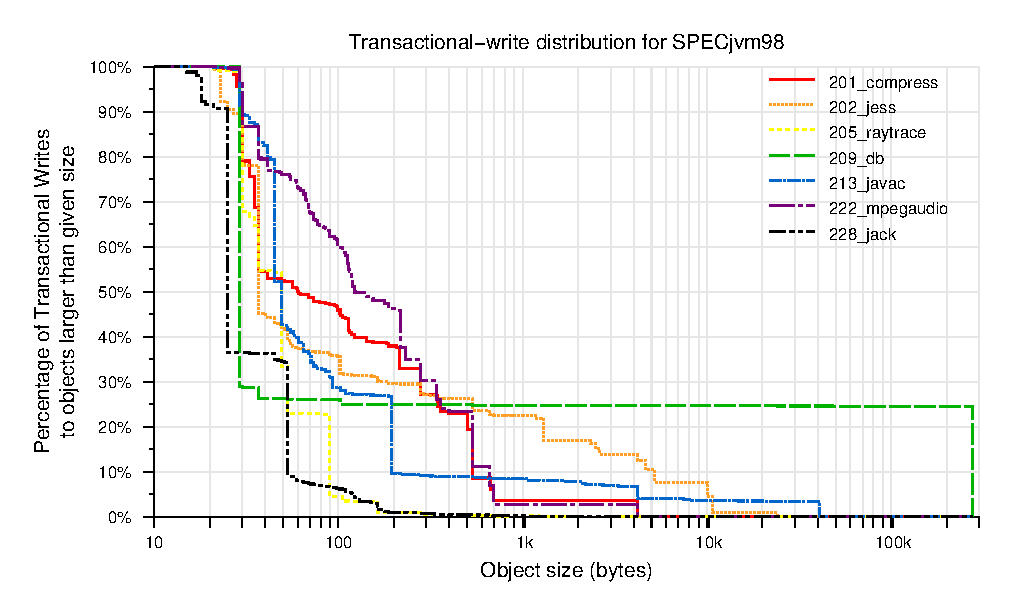
\includegraphics[height=2.75in,clip=true]{Figures/tr-w-all-1}%
\end{center}%
\caption{Proportion of transactional writes to objects equal to or
  smaller than a given size.}
\label{fig:tr-w}%
\end{figure}%
The basic \apex software transaction system clones objects on
transactional writes so that the previous state of the object can be
restored if the transaction aborts.  \figref{tr-w} shows the object
size distribution of transactional writes for SPECjvm98, and
indicates that over 10\% of writes may be to large objects.
As we've seen in \secref{full-bench}, the copying cost can become
excessive.

The solution I propose
represents objects as \defn{functional
  arrays}.  O'Neill and Burton \cite{ONeillBu97} give a fairly
inclusive overview of such algorithms; I've chosen Tyng-Ruey Chuang's
version \cite{Chuang94} of \emph{shallow binding}, which uses
randomized cuts to the version tree to limit the cost of a read to
$O(n)$ in the worst case.  Single-threaded accesses to the array run in
$O(1)$ time.  My use of functional arrays is single-threaded in the common
case when transactions do not abort.  Chuang's scheme is attractive,
because it limits the worst-case cost of an abort, with little
added complexity.

In this chapter I recast the basic \apex design of the previous
chapters as a
``small-object protocol,'' and then show how to extend it to a ``large-object protocol,'' in the process addressing the large-object performance
problems.  The large-object protocol, which we'll call \lapex, uses a
lock-free variant of 
Chuang's algorithm, which I present in \secref{lf-fun-arr}.

\section{Basic operations on functional arrays}\label{sec:naivefun}
Let us begin by reviewing the basic operations on functional arrays.
Functional arrays are \emph{persistent}; that is,
after an element is updated, both the new and the old contents of the
array are available for use.  Since arrays are simply maps from
integers (indexes) to values, any functional-map datatype (for
example, a functional balanced tree) can be used to implement
functional arrays.

In contrast, an imperative array---such as those in imperative
languages such as Java---is mutable.  Elements of the array are
updated ``in place'', destroying the old value of the element.  Only
the updated array is available for use after an update.
The distinguishing characteristic of an imperative array is its
time complexity: $O(1)$ time to access or update any element.
Implementing functional arrays with a functional balanced tree yields
$O(\lg n)$ worst-case access or update.\footnote{I return to
a discussion of operational complexity in \secref{lf-fun-arr}.}

For concreteness, a functional array defines the following three
operations:
\begin{itemize}
\item $\funcname{FA-Create}(n)$: Return an array $A$ of size $n$.  The
  contents of the array are initialized to $0$.
\item $\funcname{FA-Update}(A, i, v)$: Return an array $A'$ that is
  functionally identical to array $A$ except that
  $\funcname{FA-Read}(A', i)=v$.
  Array $A$ is not destroyed and can be accessed further.
\item $\funcname{FA-Read}(A, i)$: Return $A(i)$ (that is, the
  value of the $i$th element of array $A$).
\end{itemize}
We allow any of these operations to \emph{fail}.  Failed operations
can be safely retried, as all operations are idempotent by definition.

For the moment, consider the following \naive implementation:
\begin{itemize}
\item $\funcname{FA-Create}(n)$: Return an ordinary imperative array of size
  $n$.
\item $\funcname{FA-Update}(A, i, v)$: Create a new imperative array
  $A'$ and copy the contents of $A$ to $A'$.  Set $A'[i]=v$. Return $A'$.
\item $\funcname{FA-Read}(A, i)$: Return $A[i]$.
\end{itemize}
Since this implementation costs $O(1)$ to read and $O(n)$ to update,
it matches
the performance of imperative arrays only when $R = O(U \cdot n)$,
where $R$ is the number of reads and $U$ is the number of updates.
In most code, $R \approx 3U$ \cite[p. 105]{HennessyPa96} and the
constant factors hidden by the big-O notation are small, so the
performance equivalence is only valid when $n$ is relatively small.  I
therefore call these \emph{small-object functional arrays}.  Operations
in this implementation never fail.  Every operation is nonblocking
and no synchronization is necessary, since the imperative arrays are
never mutated after they are created.   \Secref{lf-fun-arr}
reviews better functional array implementations and presents
a new lock-free variant.

\section{A single-object protocol}
\begin{figure}\centering
\includegraphics[width=3.25in,clip=true]{Figures/nb-single-obj}
\caption{Implementing nonblocking single-object concurrent operations
  with functional arrays.}
\label{fig:single-o}
\end{figure}
Given a nonblocking implementation of functional arrays, we can
construct a transaction implementation for single objects.  In
this implementation, fields of at most one object may be referenced
during the execution of the transaction.

Consider the following two operations on objects:
\begin{itemize}
\item $\funcname{Read}(o, f)$: Read field $f$ of $o$.  Assume that
  there is a constant mapping function, which, given a field name $f$,
  returns an integer index, \fref{f}{index}.
  For simplicity and without loss of generality,
  assume that all field sizes are equal.
\item $\funcname{Write}(o, f, v)$: Write value $v$ to field $f$ of $o$.
\end{itemize}
All other operations on Java objects, such as method dispatch and type
interrogation, can be performed using the immutable {\tt type}
field in the object.  Because the {\tt type} field never changes
after object creation, implementing nonblocking operations on
the {\tt type} field is straightforward.

As Figure~\ref{fig:single-o} shows, our single-object transaction
implementation represents objects as a pair, combining {\tt type} and a
reference to a functional array.  When not inside a transaction,
object reads and writes are implemented using the
corresponding functional array operation, with the array reference in
the object being updated appropriately:
\begin{itemize}
\item $\funcname{Read}(o, f)$:
  Return $\funcname{FA-Read}(\fref{o}{fields}, \fref{f}{index})$.
\item $\funcname{Write}(o, f, v)$: Replace \fref{o}{fields} with the
  result of \linebreak
  $\funcname{FA-Update}(\fref{o}{fields}, \fref{f}{index}, v)$.
\end{itemize}

The interesting cases are reads and writes inside a transaction.
At entry to a transaction that will access (only) object $o$, the
single-object version of \lapex
stores \fref{o}{fields} in a local variable $u$.  We create another
local variable $u'$ initialized to $u$.  Then, the read and
write operations are implemented as follows:
\begin{itemize}
\item $\funcname{ReadT}(o, f)$:
  Return $\funcname{FA-Read}(u', \fref{f}{index})$.
\item $\funcname{WriteT}(o, f, v)$:
  Update variable $u'$ to the result of \linebreak
  $\funcname{FA-Update}(u', \fref{f}{index}, v)$.
\end{itemize}

At the end of the transaction, we use Compare-And-Swap to atomically
set \fref{o}{fields} to $u'$ if and only if it contained $u$.  If the CAS fails,
the transaction is aborted (we simply discard $u'$) and retried.

With our \naive ``small object'' functional arrays, this implementation is
exactly the ``small-object protocol'' of Herlihy \cite{Herlihy93}.
Herlihy's protocol is rightly criticized for an excessive amount of
copying.  I address this criticism with a better implementation of
functional arrays in \secref{lf-fun-arr}.  First, however, I remove
the restriction that only one object
may be referenced within a transaction.

\section{Extension to multiple objects}
\begin{figure}\centering
\includegraphics[width=3.25in,clip=true]{Figures/nb-multi-obj}
\caption[Data structures to support nonblocking multiobject
  concurrent operations.]{Data structures to support nonblocking multiobject
  concurrent operations.  Objects point to a linked list of versions,
  which reference transaction identifiers.  Versions created within the
  same execution of a transaction share the same transaction
  identifier.  Version structure also contain pointers to functional
  arrays, which record the values for the fields of the object.
  If no modifications have been made to the object, multiple versions
  in the list may share the same functional array.  (Compare this model
  of a transaction system to our concrete design in \figref{tr-multi-obj-big}.)}
\label{fig:multi-o}
\end{figure}
\begin{figure}
\sis\small%
\renewcommand{\>}{~~}%
\newcommand{\com}[1]{\hfill [{\sl #1}]}%
\begin{tabular}{l}%
$\funcname{Read}(o, f)$:\\
begin\\
retry:\\
\>$u \gets \fref{o}{versions}$ \\
\>$u' \gets \fref{u}{next}$ \\
\>$s  \gets \fref{\fref{u}{owner}}{status}$ \\
\>if ($s=\text{\sl DISCARDED}$) \com{Delete DISCARDED?}\\
\>\>CAS$(u, u', \addr{\fref{o}{versions}})$\\
\>\>goto retry \\
\>else if ($s=\text{\sl COMPLETE}$)\\
\>\>$a \gets \fref{u}{fields}$ \com{$u$ is COMPLETE}\\
\>\>$\fref{u}{next} \gets \text{\bf null}$ \com{Trim version list}\\
\>else\\
\>\>$a \gets \fref{u'}{fields}$ \com{$u'$ is COMPLETE}\\
\>return $\funcname{FA-Read}(a, \fref{f}{index})$ \com{Do the read}\\
end\\
\\
$\funcname{ReadT}(o, f)$:\\
begin\\
\>$u \gets \fref{o}{versions}$\\
\>if ($\var{oid} = \fref{u}{owner}$) \com{My OID should be first}\\
\>\>return $\funcname{FA-Read}(\fref{u}{fields}, \fref{f}{index})$
\com{Do the read}\\
\>else \com{Make me first!}\\
\>\>$u' \gets \fref{u}{next}$\\
\>\>$s  \gets \fref{\fref{u}{owner}}{status}$\\
\>\>if ($s=\text{\sl DISCARDED}$) \com{Delete DISCARDED?}\\
\>\>\>CAS$(u, u', \addr{\fref{o}{versions}})$\\
\>\>else if ($\fref{\var{oid}}{status}=\text{\sl DISCARDED}$)
\com{Am I alive?}\\
\>\>\>fail\\
\>\>else if ($s=\text{\sl IN-PROGRESS}$) \com{Abort IN-PROGRESS?}\\
\>\>\>CAS$(s, \text{\sl DISCARDED}, \addr{\fref{\fref{u}{owner}}{status}})$\\
\>\>else \com{Link new version in:} \\
\>\>\>$\fref{u}{next} \gets \text{\bf null}$ \com{Trim version list}\\
\>\>\>$u' \gets \text{new \tt Version}(\var{oid}, u, \text{\bf null})$
~~~~~~~~~\com{Create new version}\\
\>\>\>if (CAS$(u, u', \addr{\fref{o}{versions}}) \neq \text{\sl FAIL}$)\\
\>\>\>\>$\fref{u'}{fields} \gets \fref{u}{fields}$ \com{Copy old fields}\\
\>\>goto retry\\
end\\
\end{tabular}
\caption{\funcname{Read} and \funcname{ReadT} implementations for the
  multiobject protocol.}\label{fig:reads}
\end{figure}

\begin{figure}
\sis\small%
\renewcommand{\>}{~~}%
\newcommand{\com}[1]{\hfill [{\sl #1}]}%
\begin{tabular}{l}%
$\funcname{Write}(o, f, v)$:\\
begin\\
retry:\\
\>$u  \gets \fref{o}{versions}$\\
\>$u' \gets \fref{u}{next}$\\
\>$s  \gets \fref{\fref{u}{owner}}{status}$\\
\>if ($s=\text{\sl DISCARDED}$) \com{Delete DISCARDED?}\\
\>\>CAS$(u, u', \addr{\fref{o}{versions}})$\\
\>else if ($s=\text{\sl IN-PROGRESS}$) \com{Abort IN-PROGRESS?}\\
\>\>CAS$(s, \text{\sl DISCARDED}, \addr{\fref{\fref{u}{owner}}{status}})$\\
\>else \com{$u$ is COMPLETE}\\
\>\>$\fref{u}{next} \gets \text{\bf null}$ \com{Trim version list}\\
\>\>$a \gets \fref{u}{fields}$\\
\>\>$a' \gets \funcname{FA-Update}(a, \fref{f}{index}, v)$\\
\>\>if (CAS$(a, a', \addr{\fref{u}{fields}}) \neq \text{\sl FAIL}$)
~~~~~~~~~\com{Do the write}\\
\>\>\>return \com{Success!}\\
\>goto retry\\
end\\
\\
$\funcname{WriteT}(o, f, v)$:\\
begin\\
\>$u  \gets \fref{o}{versions}$\\
\>if ($oid = \fref{u}{owner}$) \com{My OID should be first}\\
\>\>$\fref{u}{fields} \gets \funcname{FA-Update}(\fref{u}{fields}, \fref{f}{index}, v)$\com{Do write}\\
\>else \com{Make me first!}\\
\>\>$u' \gets \fref{u}{next}$\\
\>\>$s  \gets \fref{\fref{u}{owner}}{status}$\\
\>\>if ($s=\text{\sl DISCARDED}$) \com{Delete DISCARDED?}\\
\>\>\>CAS$(u, u', \addr{\fref{o}{versions}})$\\
\>\>else if ($\fref{\var{oid}}{status}=\text{\sl DISCARDED}$)
\com{Am I alive?}\\
\>\>\>{\it fail}\\
\>\>else if ($s=\text{\sl IN-PROGRESS}$) \com{Abort IN-PROGRESS?}\\
\>\>\>CAS$(s, \text{\sl DISCARDED}, \addr{\fref{\fref{u}{owner}}{status}})$\\
\>\>else \com{Link new version in:} \\
\>\>\>$\fref{u}{next} \gets \text{\bf null}$ \com{Trim version list}\\
\>\>\>$u' \gets \text{new \tt Version}(\var{oid}, u, \text{\bf null})$
\com{Create new version}\\
\>\>\>if (CAS$(u, u', \addr{\fref{o}{versions}}) \neq \text{\sl FAIL}$)\\
\>\>\>\>$\fref{u'}{fields} \gets \fref{u}{fields}$ \com{Copy old fields}\\
\>\>goto retry\\
end\\
\end{tabular}
\caption{\funcname{Write} and \funcname{WriteT} implementations for the
  multiobject protocol.}\label{fig:writes}
\end{figure}

I extend the implementation to allow the fields of any number of
objects to be accessed during the transaction.
Figure~\ref{fig:multi-o} shows our new object representation.
Compare this figure to \figref{tr-multi-obj-big}; we've successfully
recast the basic \apex design in terms of operations on an array datatype.
Objects consist of two slots, and the first represents the immutable
{\tt type}, as before.  The second field, {\tt versions}, points to a
linked list of {\tt Version} structures.  The {\tt Version} structures
contain a pointer {\tt fields} to a functional array, and a pointer
{\tt owner} to an \emph{transaction identifier}.  The transaction
identifier contains a single field, {\tt status}, which can be set to
one of three values: \textsl{COMMITTED}, \textsl{IN-PROGRESS}, or
\textsl{ABORTED}\@.  When the transaction identifier is created, the
status field is initialized to \textsl{IN-PROGRESS}, and it will be
updated exactly once thereafter to either \textsl{COMMITTED} or
\textsl{ABORTED}\@.  A \textsl{COMMITTED} transaction identifier never
later becomes \textsl{IN-PROGRESS} or \textsl{ABORTED}, and
a \textsl{ABORTED} transaction identifier never becomes
\textsl{COMMITTED} or \textsl{IN-PROGRESS}\@.

We create an transaction identifier when we begin or restart a transaction
and place it in a local variable \emph{tid}.  At the end of the
transaction, we use CAS to set \fref{\var{tid}}{status} to
{\sl COMMITTED} if and only if it was {\sl IN-PROGRESS}\@.  If the CAS is successful,
the transaction has also executed successfully; otherwise
$\fref{\var{tid}}{status}=\text{\sl ABORTED}$ (which indicates that
our transaction has been aborted), and we must back off and retry.
All {\tt Version} structures
created while in the transaction reference \emph{tid} in
their {\tt owner} field.

Semantically, the current field values for the object are given by
the first version in 
the versions list whose transaction identifier is {\sl COMMITTED}\@.
These semantics allow us to link {\sl IN-PROGRESS} versions in at the head of
multiple objects' versions lists and atomically change the values of
all these objects by setting the one common transaction identifier to
{\sl COMMITTED}\@.  We only allow one {\sl IN-PROGRESS} version on the
versions list, and it must be at the head. Thus,
before we can link a new version at the head, we
must ensure that every other version on the list is {\sl ABORTED} or
{\sl COMMITTED}\@.

Since we never look past the first {\sl COMMITTED} version in the
versions list, we can free all versions past that point.  In our
presentation of the algorithm, we do this deallocation by explicitly setting the
{\tt next} field of every {\sl COMMITTED} version we see to {\bf null};
overwriting the reference allows the versions past that point to be garbage collected.
An optimization is for the garbage collector to do the list
trimming for us when it does a collection.

% always must read u.next before u.owner.status to ensure we don't
% get caught with a null pointer from a version that just committed.

Because we don't want to inadvertently chase the null {\tt next} pointer
of a {\sl COMMITTED} version, we always load the {\tt next}
field of a version \emph{before} we load {\tt owner.status}.  Since
the writes occur in the reverse order ({\sl COMMITTED} to
{\tt owner.status}, then {\bf null} to {\tt next}), we have ensured that
our {\tt next} pointer is valid whenever the status is not {\sl COMMITTED}\@.

We begin an atomic method with \funcname{TransStart} and attempt to
complete an atomic method with \funcname{TransEnd}.  They are defined as
follows:
\begin{itemize}
\item $\funcname{TransStart}$: create a new transaction identifier with
  its status initialized to {\sl IN-PROGRESS}\@.  Assign it to the
  thread-local variable \var{tid}.
\item $\funcname{TransEnd}$:
  If
 $$\text{CAS}(\text{\sl IN-PROGRESS}, \text{\sl COMMITTED},
             \addr{\fref{\var{tid}}{status}})$$
  is successful, the transaction as a whole has completed successfully
  and can be linearized at the location of the CAS\@.
  Otherwise, the transaction has been aborted.  Back off and retry from
  \funcname{TransStart}.
\end{itemize}
Pseudocode describing \funcname{Read}, \funcname{Write}, \funcname{ReadT},
and \funcname{WriteT} is presented in Figures~\ref{fig:reads} and
\ref{fig:writes}.  In the absence of contention, all operations take
constant time plus an invocation of \funcname{FA-Read} or
\funcname{FA-Update}.

\section{Lock-free functional arrays}\label{sec:lf-fun-arr}
\begin{figure}[tp]\centering
\includegraphics[width=5in,clip=true]{Figures/chuang-trim}
\caption[Shallow binding scheme for functional arrays.]
  {Shallow binding scheme for functional arrays
  \cite[Figure~1]{Chuang94}.  The array is of size 2 and is indexed by
  $x$ and $y$.  The initial array $A$ is undefined, and $B$ is defined
  as an update to $A$ at index $x$ by value $0$.  Similarly for $C$
  and $D$.  The dark node is the root node which has the cache.  White
  nodes are differential nodes which must first be rerooted before
  being read.  Note that only the root node has the cache.}
\label{fig:chuang}
\end{figure}
This section presents a lock-free implementation of functional
arrays with $O(1)$ performance for both read and update in the absence of contention.
The crucial operation is a rotation of a \emph{difference node} with the
main body of the array. Using this implementation of functional arrays
in the multiobject transaction protocol of the previous section
creates \lapex, our reimplementation of nonblocking transactions which
solves the large-object problem.

Let's begin by reviewing the well-known functional array
implementations.  As mentioned previously,
O'Neill and Burton \cite{ONeillBu97} give an
inclusive overview.  Functional array implementations fall generally
into one of three categories: \emph{tree-based}, \emph{fat-elements},
or \emph{shallow-binding}.

Tree-based implementations typically have a logarithmic term in their
complexity.  The simplest is the persistent binary tree with $O(\ln
n)$ look-up time; Chris Okasaki 
\cite{Okasaki95} has implemented a purely functional random-access list
with $O(\ln i)$ expected lookup time, where $i$ is the index of the
desired element.

Fat-elements implementations have per-element data structures indexed
by a master array. Cohen \cite{Cohen84} hangs a list of
versions from each element in the master array.
O'Neill and Burton \cite{ONeillBu97}, in a more sophisticated
technique, hang a splay tree off each element and achieve $O(1)$
operations for single-threaded use, $O(1)$ amortized cost when
accesses to the array are ``uniform'', and $O(\ln n)$ amortized worst
case time. 

Shallow binding was introduced by Baker \cite{Baker78} as a method to
achieve fast variable lookup in Lisp environments.  Baker clarified
the relationship to functional arrays in \cite{Baker91}.  Shallow
binding is also called \emph{version tree arrays}, \emph{trailer
  arrays}, or \emph{reversible differential lists}.  A typical
drawback of shallow binding is that reads may take $O(u)$ worst-case
time, where $u$ is the number of updates made to the array.  Tyng-Ruey
Chuang \cite{Chuang94} uses randomized cuts to the version tree to limit
the cost of a read to $O(n)$ in the worst case.  Single-threaded
accesses are $O(1)$.

Our use of functional arrays is single-threaded in the common case,
when transactions do not abort.  Chuang's scheme is attractive because
it limits the worst-case cost of an abort with little added
complexity.   In this section I will present a lock-free version of
Chuang's randomized algorithm.

In shallow binding, only one version of the functional array (the
\emph{root}) keeps its contents in an imperative array (the
\emph{cache}).   Each of the other versions is represented as a path
of \emph{differential nodes}, where each node describes the
differences between the current array and the previous array.  The
difference is represented as a pair \tuple{\text{\it index},\text{\it value}},
representing the new value to be stored at the specified index.
All paths lead to the root.  An update to the functional array is
simply implemented by adding a differential node pointing to the array it is
updating.

The key to constant-time access for single-threaded use is provided by the read
operation.  A read to the root simply reads the appropriate value from
the cache.  A read to a differential node, however, triggers a series
of rotations that swap the direction of differential nodes and result
in the current array acquiring the cache and becoming the new root.
This sequence of rotations is called \emph{rerooting}, and is
illustrated in Figure~\ref{fig:chuang}.  Each rotation
exchanges the root nodes for a differential node pointing to it, after
which the differential node becomes the new root and the root becomes
a differential node pointing to the new root. The cost of a read is
proportional to its rerooting length, but after the first read
accesses to the same version are $O(1)$ until the array is rerooted again.

Shallow binding performs badly if read operations ping-pong between two
widely separated versions of the array, as we will continually
reroot the array from one version to the other.
Chuang's contribution is to provide for \emph{cuts} to the chain of
differential nodes: once in a while we clone the cache and create a
new root instead of performing a rotation.  Since this operation takes
$O(n)$ time, we amortize it over $n$ operations by randomly
choosing to perform a cut with probability $1/n$.

\begin{figure}\centering%
\includegraphics[width=5in,clip=true]{Figures/funarr}
\caption[Atomic steps in $\funcname{FA-Rotate}(B)$.]%
 {Atomic steps in $\funcname{FA-Rotate}(B)$.  Time proceeds top-to-bottom
  on the left hand side, and then top-to-bottom on the right.
  Array $A$ is a root node, and $\funcname{FA-Read}(A, x)=z$.
  Array $B$ has the almost the same contents as $A$, but
  $\funcname{FA-Read}(B, x)=y$.}
\label{fig:funarr}
\end{figure}

\begin{figure}\centering%
\sis%
\renewcommand{\>}{~~}%
\newcommand{\com}[1]{\hfill [{\sl #1}]}%
\begin{tabular}{l}%
$\funcname{FA-Update}(A, i, v)$:\\
begin\\
\>$d \gets \text{new DiffNode}(i, v, A)$\\
\>$A'\gets \text{new Array}(\fref{A}{size}, d)$\\
\>return $A'$\\
end\\
\\
$\funcname{FA-Read}(A, i)$:\\
begin\\
retry:\\
\>$d_C \gets \fref{A}{node}$\\
\>if $d_C$ is a cache, then\\
\>\>$v \gets \fref{A}{node}[i]$\\
\>\>if $(\fref{A}{node} \neq d_C)$\com{consistency check}\\
\>\>\>goto retry\\
\>\>return $v$\\
\>else\\
\>\>\funcname{FA-Rotate}(A)\\
\>\>goto retry\\
end\\
\end{tabular}
\caption{Implementation of lock-free functional array using shallow
  binding and randomized cuts (part 1).}
\label{fig:fun-impl1}
\end{figure}
\begin{figure}\centering%
\sis%
\renewcommand{\>}{~~}%
\newcommand{\com}[1]{\hfill [{\sl #1}]}%
\begin{tabular}{l}%
$\funcname{FA-Rotate}(B)$:\\
begin\\
retry:\\
\>$d_B \gets \fref{B}{node}$\com{step (1): assign names as per Figure~\ref{fig:funarr}.}\\
\>$A \gets \fref{d_B}{array}$\\
\>$x \gets \fref{d_B}{index}$\\
\>$y \gets \fref{d_B}{value}$\\
\>$z \gets \funcname{FA-Read}(A, x)$\com{rotates A as side effect}\\
\\
\>$d_C \gets \fref{A}{node}$\\
\>if $d_C$ is not a cache, then \\
\>\>goto retry\\
\\
\>if $(0 = (\text{random} \bmod \fref{A}{size}))$\com{random cut}\\
\>\>$d_C' \gets \text{copy of }d_C$\\
\>\>$d_C'[x] \gets y$\\
\>\>$s\gets\text{DCAS}(d_C, d_C, \addr{\fref{A}{node}}, d_B, d_C', \addr{\fref{B}{node}})$\\
\>\>if $(s \neq \text{\sl SUCCESS})$ goto retry\\
\>\>else return\\
\\
\>$C \gets \text{new Array}(\fref{A}{size}, d_C)$\\
\>$d_A \gets \text{new DiffNode}(x, z, C)$\\
\\
\>$s \gets \text{CAS}(d_C, d_A, \addr{\fref{A}{node}})$\com{step (2)}\\
\>if $(s\neq \text{\sl SUCCESS})$ goto retry\\
%\\
\>$s\gets\text{CAS}(A, C, \addr{\fref{d_B}{array}})$\com{step (3)}\\
\>if $(s\neq \text{\sl SUCCESS})$ goto retry\\
%\\
\>$s \gets\text{CAS}(C, B, \addr{\fref{d_A}{array}})$\com{step (4)}\\
\>if $(s\neq \text{\sl SUCCESS})$ goto retry\\
%\\
\>$s \gets \text{DCAS}(z, y, \addr{d_C[x]},  d_C, d_C, \addr{\fref{C}{node}})$\com{step (5)}\\
\>if $(s\neq \text{\sl SUCCESS})$ goto retry\\
%\\
\>$s \gets \text{DCAS}(d_B, d_C, \addr{\fref{B}{node}}, d_C, {\bf nil}, \addr{\fref{C}{node}})$\com{step (6)}\\
\>if $(s\neq \text{\sl SUCCESS})$ goto retry\\
end\\
\end{tabular}
\caption{Implementation of lock-free functional array using shallow
  binding and randomized cuts (part 2).}
\label{fig:fun-impl2}
\end{figure}

Figure~\ref{fig:funarr} shows the data structures used for the
functional array implementation, as well as the series of atomic steps used
to implement a rotation.  The {\tt Array} class, which represents a
functional array, consists of a {\tt size} for the array and a
pointer to a {\tt Node}.  There are two types of nodes: a {\tt
  CacheNode} stores a value for every index in the array, whereas a {\tt
  DiffNode} stores a single change to an array.  {\tt Array} objects
that point to {\tt CacheNode}s are roots.

In step 1 of the figure, we have a root array $A$ and an
array $B$ whose differential node $d_B$ points to $A$.  The functional
arrays $A$ and $B$ differ in one element: element $x$ of $A$ is $z$,
while element $x$ of $B$ is $y$.  We are about to rotate $B$ to give
it the cache, while linking a differential node to $A$.

Step 2 shows our first atomic action.  We have created a new {\tt
  DiffNode} $d_A$ and a new {\tt Array} $C$ and linked them between
$A$ and its cache.  The {\tt DiffNode} $d_A$ contains the value for
element $x$ contained in the cache, $z$, so there is no change in
the value of $A$.

We continue swinging pointers until step 5, when we can finally set
the element $x$ in the cache to $y$.  We perform this operation with a
DCAS operation that checks that $\fref{C}{node}$ is still pointing to
the cache as we expect.  A concurrent rotation would swing
$\fref{C}{node}$ in its step 1.  In general, therefore, the location
pointing to the cache serves as a reservation on the cache.

Thus, in step 6 we need to again use DCAS to simultaneously swing
$\fref{C}{node}$ away 
from the cache as we swing $\fref{B}{node}$ to point to the cache.

Figures~\ref{fig:fun-impl1} and \ref{fig:fun-impl2} present pseudocode
for \funcname{FA-Rotate}, \funcname{FA-Read}, and
\funcname{FA-Update}.  Like \funcname{FA-Rotate}, \funcname{FA-Read} procedure also uses the
cache pointer as a reservation, double-checking the cache pointer
after it finishes its read to ensure that the cache hasn't been stolen
from it.

Let us now consider cuts, where \funcname{FA-Read} clones the cache
instead of performing a rotation.   Cuts also check the cache pointer
to protect against concurrent rotations.  But, what if the cut occurs
while a rotation is mutating the cache in step 5?  In this case, because the
only array adjacent to the root is $B$, the cut must be occurring
during an invocation of $\funcname{FA-Rotate}(B)$, in which case the
differential node $d_B$ will be applied after the cache is copied,
thereby safely overwriting the mutation we were concerned about.

With hardware support for small transactions \cite{HerlihyMo93}
we could cheaply perform the entire rotation atomically, instead of
using this six-step approach.


%% \section{Optimizations}
%% Rerooting is the most complicated part of the functional array
%% algorithm.  It can be optimized in several ways.  For example,

%% %unsync rotate for transaction-local data.
%% The first is to recognize that some array versions can only be seen by
%% a single thread.  In particular, when we are working on an {\sl
%%   IN-PROGRESS} operation, all array versions which it creates are
%% unreachable from other threads until the operation is committed.
%% We can add a field {\tt creator} to the {\tt Array} object that records what
%% operation created that version.  If the {\tt creator} field of both
%% $A$ and $B$ contains our own \var{tid} when we begin a rotate, we know
%% that these versions are both thread local

%% .. uh, no.  This doesn't work.

%% % scales method of tagging fields.

\section{Performance of functional array implementations}
This section presents performance measurements for our lock-free functional
array implementation using a simple read/update microbenchmark.  We
compare our lock-free functional arrays with imperative arrays, \naive
functional arrays (\secref{naivefun}), shallow-binding functional
arrays \cite{Baker91}, and Chuang's randomized-cut shallow-binding
functional arrays \cite{Chuang94}.

\begin{figure}
\sis\fontsize{9}{10}\begin{verbatim}
#define REPETITIONS 100000
typedef int32_t field_t;
typedef int32_t index_t;

void do_bench(struct aarray *obj, index_t len) {
  int i, j;

  /** Initialize the array */
  for (i=0; i<len; i++)
    obj = write(obj, i, i);
  /** Now reverse the array many times. */
  for (j=0; j<(REPETITIONS*2); j++) {
#if defined(SINGLETHREAD) // single-threaded access
    for (i=0; i<len/2; i++) {
      field_t v1 = read(obj, i);
      field_t v2 = read(obj, len-i-1);
      obj = write(obj, i, v2);
      obj = write(obj, len-i-1, v1);
    }
#else // multi-threaded access
    struct aarray *robj = obj;
    for (i=0; i<len; i++)
      obj = write(obj, len-i-1, read(robj, i));
#endif
  }
  /** Check that the array has the expected values */
  for (i=0; i<len; i++)
    assert(read(obj, i)==i);
}
\end{verbatim}
\caption{Array reversal microbenchmark to evaluate performance of
  functional array implementations.}
\label{fig:array-bench}
\end{figure}

\figref{array-bench} shows the basic structure of the microbenchmark.
The \texttt{read()} and \texttt{write()} methods
have appropriate definitions inlined for each variant of the
benchmark.  This microbenchmark is patterned after that used in
\cite[p.507]{ONeillBu97}.  With \texttt{SINGLETHREAD} defined,
accesses are imperative or ``single-threaded''---only the latest
version of the array is referenced.  The algorithm corresponds to the
typical imperative array reversal algorithm.  We swap the leftmost and
rightmost element of the array and move inward as we continue to swap.
Without \texttt{SINGLETHREAD} defined,
the reversal algorithm always reads from the original
array.  This pattern of access corresponds to a frequent abort scenario.
In our experiments the single-threaded and multi-threaded variants of
the benchmark had almost identical performance, contrary to the claims
of \cite{ONeillBu97}.  Standard shallow-binding will have poor
performance only if reads of the half-reversed array were to occur in the
multi-threaded variant.  These reads are not necessary for array reversal.

\epsbigfigput[Functional array performance on an array reversal microbenchmark.]{phd-arrayperf}{Functional array performance on an
  array reversal microbenchmark as the size of the array is varied.
  Both axes are logarithmic.  The y axis shows the average time, in
  nanoseconds, required to do an array read followed by an update.
  The benchmark initialized the array and then reversed its contents
  200,000 times.  The reversal swapped the
  first and last elements, then the second and second-to-last
  elements, etc.}

\figref{phd-arrayperf} shows the performance of various array
implementations using the single-threaded variant of the benchmark.
I measured the number of microseconds required for a read and update pair
on the array, as the size of the array ranged from 8 to 4096 elements.
Benchmarks were executed on the PowerPC hardware described in
\secref{full-bench}.\footnote{Results on a 1.4GHz Pentium M were similar.}

Standard imperative arrays averaged 5.0 nanoseconds per read-update,
mostly invariant with array size.  The \naive functional array
implementation, described in \secref{naivefun}, ranged from 475 ns
for 8-element arrays up to 47,629 ns for 4096-element arrays.  The
exponential growth in run time with increasing array size demonstrates the
``large object problem'' which motivated our investigation of
lock-free functional arrays in this chapter.

Shallow-binding functional arrays \cite{Baker91} averaged 327
nanoseconds per read-update.  This is over 60 times slower than
standard imperative arrays, but is invariant with array size.
Shallow binding shows poor performance when accesses are not
single-threaded---or when transactions abort often, in a transactional
application.

Chuang's randomized-cut shallow-binding functional arrays
\cite{Chuang94}, labeled ``Random Cut'' in \figref{phd-arrayperf},
allow good performance even when transactions abort
often.  My implementation averaged 400 ns per read-update.  The
root-cloning which allows multi-threaded access imposes an additional
22\% overhead when compared to the standard shallow binding functional
array implementation.

Finally, my lock-free version of Chuang's functional arrays, labeled
``Lock-Free'', averages
894 ns per read-update.  The penalty for performing the lock-free
algorithm is 124\%, resulting in read-updates which are over 175 times slower
than imperative array read-updates.   \figref{phd-arrayperf} shows
that the lock free algorithm is still faster than copying objects on
update when the objects are larger than 32 words long.

In a hybrid transaction system which used small hardware transaction
support for the functional array implementation, one could expect
performance similar to the standard randomized-cut shallow-binding
implementation.  One would simply make the rotation operations atomic
using the hardware transaction system.

%%%%%%%%%%%%%%%%%%%%%


% LocalWords:  Promela microbenchmark Hennessy PowerPC setjmp longjmp runtime
% LocalWords:  subsumption TransactionAbortException mutex unsynchronized gzip
% LocalWords:  SPECjvm multithreaded transactified Transactification renderer
% LocalWords:  javac analyses StringBuffer stwcx transactionally ReaderList gcc
% LocalWords:  readNT writeNT readT writeT ensureWriter checkWriteField inlined
% LocalWords:  inlines inline PowerPC's Sparc StrongARM Classpath backend JNI
% LocalWords:  bytecode desugaring ensureReader desugar superclass NaN JDK jess
% LocalWords:  parameterized datatype Herlihy ensureReader nontransactional UTM
% LocalWords:  transactification mpegaudio raytrace LTM microarchitecture RISC
% LocalWords:  backoff syscall livelock subword subwords lookup Chuang
% LocalWords:  nonblocking Herlihy's Pseudocode
